\documentclass[twocolumn, 10pt]{article}

\usepackage{amsmath}
\usepackage{amssymb}
\usepackage{booktabs}
\usepackage{graphicx}
\usepackage[colorlinks=true, citecolor=blue, linkcolor=blue, urlcolor=blue]{hyperref}
\usepackage{xcolor}
\usepackage[round]{natbib}
\usepackage[margin=1in]{geometry}

% Astronomy-style degree/arcmin/arcsec
% These commands work both in text and math mode
\newcommand{\arcsec}{\ensuremath{^{\prime\prime}}}
\newcommand{\arcmin}{\ensuremath{^{\prime}}}
\newcommand{\degr}{\ensuremath{^{\circ}}}

\begin{document}

\title{Zodiacal: Accelerating Blind Astrometric Plate Solving Through\\Multi-Scale Index Sharding}

\author{Matthew Goodman\\
\textit{Exclosure}\\
\texttt{matt@exclosure.io}}

\begin{abstract}
We present Zodiacal, a pure-Rust implementation of blind astrometric plate
solving that achieves 98.3\% solve rates on simulated narrow-field imagery
with a median solve time of 1.42\,s. Zodiacal implements the geometric hashing
framework of \citet{lang2010}, constructing scale-invariant four-star asterism
codes and matching them against prebuilt index files via $k$-d tree search.
Our primary contribution is a systematic analysis of \emph{index sharding
strategies}---the partitioning of the quad code space into narrow angular-scale
bands---and their effect on solver performance. We show that splitting a single
broadband index (10--600\arcsec) into 12 narrow bands at a $\sqrt{2}$ scale
factor increases the solve rate from 96.0\% to 98.3\% compared to 4
wider bands at a $3\times$ factor, while reducing the mean verification
count by 33\%. The improvement arises from smaller $k$-d trees per band
that reduce false-positive code matches, combined with per-index scale
filtering that skips irrelevant bands entirely. We characterize the
remaining 1.7\% failure population as
quad-matching timeouts concentrated at moderate Galactic latitudes
($|b| \approx 20$--$45\degr$), where code-space collisions create a
false-match flood. The system is fully open-source and designed for
integration into automated survey pipelines.
\end{abstract}

\date{}
\maketitle

\noindent\textbf{Keywords:} astrometry --- methods: data analysis --- techniques: image processing --- catalogs

% =============================================================================
\section{Introduction} \label{sec:intro}
% =============================================================================

Blind astrometric plate solving---the determination of a celestial image's
pointing, rotation, and plate scale from the star pattern alone---is a
foundational capability for astronomical survey pipelines, robotic telescopes,
and spacecraft attitude determination. The problem is computationally
challenging: given $N$ detected sources in an image and a catalog of $\sim10^8$
reference stars, one must identify the correct correspondence without prior
knowledge of the field's location on the sky.

The dominant approach, introduced by \citet{lang2010} and implemented in the
widely-used \texttt{astrometry.net} system, reformulates the problem as
geometric hashing. Four-star asterisms (``quads'') are encoded into a
low-dimensional code space that is invariant to rotation, scale, and parity.
A $k$-d tree indexes the code space, enabling sub-linear lookup of candidate
matches. Bayesian verification then scores each candidate World Coordinate
System (WCS) against the full star field.

While \texttt{astrometry.net} has proven highly effective---reporting
$>99.9\%$ solve rates on Sloan Digital Sky Survey (SDSS) fields
\citep{lang2010}---its implementation is distributed across C, Python, and
multiple FITS-based intermediate file formats, making it difficult to embed in
modern compiled pipelines. More importantly, the interaction between index
construction parameters and solver performance has not been systematically
characterized. In particular, the choice of how to \emph{shard} the angular
scale space into multiple index files---how many bands, how wide, and at what
scale factor---has a first-order effect on solve speed and reliability that is
not well-documented in the literature.

In this paper we present Zodiacal, a pure-Rust reimplementation of the
geometric hashing approach that achieves comparable solve rates while enabling
systematic experimentation with index construction. Our primary contribution
is an empirical analysis of index sharding strategies and their performance
implications. We demonstrate that:

\begin{enumerate}
    \item Narrower angular-scale bands reduce the effective $k$-d tree size
          per index, cutting false-positive matches and improving solve speed.
    \item Per-index scale filtering---skipping indexes whose band cannot
          overlap with the inferred backbone angular scale---provides an
          efficient pruning mechanism that scales with the number of bands.
    \item The combination of these effects yields a Pareto improvement:
          finer sharding increases both solve rate and reduces median solve
          time for the majority of fields.
    \item The residual failure population ($\sim$1.7\%) is dominated by
          code-space collisions at moderate Galactic latitudes, a regime
          where narrower bands provide diminishing returns.
\end{enumerate}

Section~\ref{sec:algorithm} describes the solver architecture.
Section~\ref{sec:indexing} details the index construction pipeline and
sharding strategies. Section~\ref{sec:results} presents benchmark results
across configurations. Section~\ref{sec:failure} analyzes the failure
population. Section~\ref{sec:discussion} discusses implications and future
work. Section~\ref{sec:bundle} extends the scale-only sharding of
\S\ref{sec:indexing} along a second, spatial axis (the
\texttt{.zdcl.bundle} format) and characterises region-restricted
solving against a depth-9, $G \le 20$ Gaia bundle.
Section~\ref{sec:pm} describes how proper motion is applied at WCS
fit and verification so that out-of-epoch plates (e.g.\ archival
Hubble frames) solve against the same Gaia-epoch bundle.

% =============================================================================
\section{Algorithm} \label{sec:algorithm}
% =============================================================================

Zodiacal implements the full pipeline described by \citet{lang2010}:
source extraction, quad formation, code matching, WCS fitting, and
Bayesian verification. We summarize each stage, noting implementation
choices that differ from \texttt{astrometry.net}.

\subsection{Source Extraction} \label{sec:extraction}

Sources are detected using a DAO/IRAF-style algorithm provided by the
\texttt{starfield} library \citep{starfield}: Gaussian convolution for
background estimation, connected-component labeling above a signal-to-noise
threshold, and flux-weighted centroiding. The result is an ordered list of
$(x, y, f)$ tuples sorted by decreasing flux $f$.

For pre-extracted source lists (e.g., from upstream pipelines), Zodiacal
accepts a JSON interchange format containing pixel positions, fluxes, and
optional metadata (known RA/Dec, plate scale hints) that can constrain the
search space.

\subsection{Quad Codec} \label{sec:codec}

A quad consists of four stars $(A, B, C, D)$. Stars $A$ and $B$ form the
\emph{backbone}---the pair with the largest angular separation among the
four. The remaining stars $C$ and $D$ are encoded relative to the backbone
in a rotation- and scale-invariant coordinate system.

Specifically, let $\mathbf{M}$ be the midpoint of $A$ and $B$ on the unit
sphere. All four stars are projected onto the tangent plane at $\mathbf{M}$
via gnomonic projection. A rotation and scaling are applied to normalize
the baseline $\overline{AB}$ to unit length along the $x$-axis, with $A$
at the origin. The positions of $C$ and $D$ in this frame yield a
four-dimensional code:
\begin{equation} \label{eq:code}
    \mathbf{c} = (c_x, c_y, d_x, d_y) \in \mathbb{R}^4.
\end{equation}

Two canonicalization invariants ensure that equivalent geometric
configurations produce identical codes regardless of labeling:
\begin{enumerate}
    \item \textbf{Mean-$x$ constraint}: if the mean of the $x$-coordinates
          exceeds 0.5, swap $A \leftrightarrow B$ and transform
          $c_i \leftarrow 1 - c_i$ for all $i$.
    \item \textbf{Ordering constraint}: sort $C$ and $D$ by their
          $x$-coordinates so that $c_x \leq d_x$.
\end{enumerate}

This codec is identical to the one described in \citet{lang2010} and
implemented in \texttt{astrometry.net}'s \texttt{quad-utils.c}.

\subsection{Two-Phase Quad Generation} \label{sec:twophase}

Field quads are generated incrementally from the $N$ brightest sources
(default $N=50$), following the two-phase strategy from
\texttt{astrometry.net}. When star $n$ is introduced:

\begin{itemize}
    \item \textbf{Phase 1}: Star $n$ serves as backbone star $B$. For each
          $A < n$, candidates $C$ and $D$ are drawn from $\{0, \ldots, n-1\}$
          within the bounding circle of the $AB$ pair.
    \item \textbf{Phase 2}: Star $n$ serves as off-diagonal star $C$. For
          each backbone pair $A < B < n$, candidate $D$ is drawn from
          $\{0, \ldots, n-1\}$.
\end{itemize}

This ensures each unique quad is attempted exactly once across all
iterations, maximizing search coverage without redundancy. A bounding
circle constraint (\S\ref{sec:abcircle}) rejects geometrically
implausible $C$ and $D$ candidates early.

\subsection{The AB-Diameter Inscription Test} \label{sec:abcircle}

The Lang quad invariant requires the two off-diagonal stars $C$ and
$D$ to lie inside the \emph{$AB$-diameter circle}---the circle whose
diameter is the segment $\overline{AB}$. In the canonical code-space
coordinates of \S\ref{sec:codec} (with $A$ at the origin and $B$ at
$(1, 0)$), this is the circle of radius $\tfrac{1}{2}$ centred on
$(\tfrac{1}{2}, \tfrac{1}{2})$:
\begin{equation} \label{eq:inbox}
    \left( x - \tfrac{1}{2}\right)^{\!2}
    + \left( y - \tfrac{1}{2}\right)^{\!2} \le \tfrac{1}{2},
\end{equation}
matching \texttt{astrometry.net}'s
\texttt{solver/quad-builder.c::check\_inbox}. During quad
\emph{construction} the test is evaluated on the sphere before
projection, to skip the gnomonic step for candidates that will fail
the invariant. Let $\mathbf{M}$ be the midpoint of $A$ and $B$ on the
unit sphere and $\theta_{AB}$ the angular separation of $A$ and $B$.
The spherical-geometry form of Eq.~\ref{eq:inbox} is
\begin{equation} \label{eq:inbox-sphere}
    \|\mathbf{C} - \mathbf{M}\|^{2} \le 2\!\left(1 - \cos\frac{\theta_{AB}}{2}\right),
\end{equation}
expressed in the squared Euclidean (chord) distance between unit
vectors. The right-hand side is the chord$^{2}$ corresponding to
angular distance $\theta_{AB}/2$ from $\mathbf{M}$, i.e. the radius
of the inscription circle on the sphere.

A subtle error in our original implementation used
$2(1 - \cos\theta_{AB})$ for the threshold---the chord$^{2}$ for
angular distance $\theta_{AB}$, twice the correct radius---admitting
candidates anywhere within distance $|\overline{AB}|$ of
$\mathbf{M}$ rather than $|\overline{AB}|/2$. The encoding-side
canonicalisation (mean-$x$ and ordering constraints of
\S\ref{sec:codec}) was unaffected, so codes themselves remained
well-formed, but the index admitted quads whose $C$ or $D$ projected
outside the validity circle in code space. The bug was caught
visually on a Hubble Space Telescope scene render where $D$ sat at
122.7\,\% of the inscription radius despite a correct solve, and
fixed by replacing the threshold with Eq.~\ref{eq:inbox-sphere} at
all three quad-build sites. Bundles rebuilt against the corrected
threshold are 20--30\,\% smaller per band, with proportionally fewer
spurious code matches per solve; older bundles continue to work
unchanged because the verifier already rejects the laxer quads as
verification failures.

\subsection{Code Matching via $k$-d Tree} \label{sec:matching}

Each prebuilt index file contains a $k$-d tree over the four-dimensional
code space of its constituent quads. Given a field code $\mathbf{c}_f$,
the solver performs a range search:
\begin{equation}
    \mathcal{M} = \left\{ \mathbf{c}_i \in \mathcal{T} :
    \|\mathbf{c}_f - \mathbf{c}_i\|^2 < \epsilon \right\},
\end{equation}
where $\mathcal{T}$ is the code tree and $\epsilon = 0.01$ is the default
squared Euclidean tolerance. Each match yields a star correspondence
$(A_f, B_f, C_f, D_f) \leftrightarrow (A_i, B_i, C_i, D_i)$.

To handle image parity (flipped fields), each field code is tried in both
the original and $x/y$-swapped orientation, doubling the match attempts
without doubling the index size.

\subsection{WCS Fitting} \label{sec:fitting}

From each four-star correspondence, a tangent-plane (TAN) WCS is fit via
least-squares. The tangent point is the centroid of the matched reference
stars' unit vectors, and the CD matrix is solved from the $2 \times 2$
normal equations relating gnomonic-projected sky coordinates to pixel
coordinates. Solutions with a singular or near-singular matrix
($|\det| < 10^{-30}$) are rejected. A residual check ensures all four
quad stars project to within 10\,pixels of their detected positions.

\subsection{Bayesian Verification} \label{sec:verify}

Following \citet{lang2010}, each candidate WCS is scored using a
Bayesian log-odds framework. Reference stars within the projected field
of view are identified via a 3D $k$-d tree range search, then projected
to pixel coordinates. A 2D $k$-d tree over the projected positions enables
efficient nearest-neighbor queries.

For each field source $s_i$, the log-odds contribution is:
\begin{equation} \label{eq:logodds}
    \Delta_i = \max\left(\log \frac{p_{\text{fg}}(s_i)}{p_{\text{bg}}},\;
    \log \frac{p_{\text{dist}}(s_i)}{p_{\text{bg}}} \right) -
    \log p_{\text{bg}},
\end{equation}
where $p_{\text{fg}}$ is a Gaussian likelihood for a genuine match
(with $\sigma = r_{\text{match}} / 2$, default $r_{\text{match}} = 5$\,px),
$p_{\text{bg}}$ is a uniform background rate, and $p_{\text{dist}}$
models a dynamic distractor rate that adapts as matches accumulate.

A solution is accepted when the cumulative log-odds exceeds 20 (odds
ratio $\sim e^{20} \approx 5 \times 10^8$:1) with at least 10 matched
stars. Early termination at log-odds $< -20$ avoids wasting time on
clearly spurious candidates.

% =============================================================================
\section{Index Construction and Sharding} \label{sec:indexing}
% =============================================================================

The quality and structure of prebuilt index files have a dominant effect
on solver performance. This section describes the index construction
pipeline and introduces the sharding strategies we evaluate.

\subsection{HEALPix Uniformization} \label{sec:healpix}

Raw star catalogs (e.g., Gaia DR3) exhibit orders-of-magnitude variation
in stellar density between the Galactic plane and poles. Naive quad
generation from such catalogs concentrates quads in dense regions, leaving
sparse regions underrepresented.

We uniformize the catalog using HEALPix \citep{gorski2005} pixelization in the
nested indexing scheme. The sky is divided into $12 \times N_{\text{side}}^2$
equal-area cells, where $N_{\text{side}} = 2^d$ at depth $d$. The depth
is automatically computed from the index's upper scale bound:
\begin{equation}
    d = \left\lceil \log_2 \frac{\sqrt{\pi/3}}{\theta_{\max}} \right\rceil,
\end{equation}
where $\theta_{\max}$ is twice the upper angular scale (in radians),
capped at $d \leq 8$ (786{,}432 cells) for memory efficiency.

For each cell, a max-heap retains only the $k$ brightest stars (default
$k = 30$), producing a spatially uniform subset of the input catalog.
This is a streaming single-pass algorithm over the catalog.

\subsection{Per-Cell Quad Building} \label{sec:percell}

Quads are generated per HEALPix cell (at a potentially different depth
than the uniformization depth). For each cell, we collect stars from the
cell and its 8 neighbors (to avoid boundary effects), build a 3D $k$-d
tree, and generate quads whose backbone angular distance falls within
$[\theta_{\min}, \theta_{\max}]$.

Key parameters controlling quad density:
\begin{itemize}
    \item \textbf{Passes} (default 16): number of quad-building sweeps
          per cell.
    \item \textbf{Max reuse} (default 8): maximum number of quads in
          which any single star may appear, enforced via atomic counters.
    \item \textbf{Max quads}: global cap, distributed uniformly across
          cells.
\end{itemize}

Quad generation is parallelized across cells using \texttt{rayon} with
an atomic done-flag for early termination when the global quota is met.

\subsection{Sky-Uniform Coverage at Depth} \label{sec:uniform}

Per-cell quad building (\S\ref{sec:percell}) achieves spatial uniformity
\emph{by design}, but only if the iteration order of the construction
loop respects the cell partition. Our initial production builder
(\texttt{src/index/builder.rs}) sorted the entire post-uniformization
catalog by brightness and emitted quads anchor-by-anchor under a single
global \texttt{max\_quads} cap. In dense regions a single bright anchor
can emit $\mathcal{O}(K^2)$ quads with $K \sim 10^2$ neighbors, so the
global cap saturates within the first few thousand anchors and faint
anchors in sparse cells never get visited. The empirical cost is severe:
on our \texttt{gaia\_g14.zdcl} production index (1\,M quads, 16.8\,M
stars at $G \le 14$), only \textbf{133 of 12{,}288} HEALPix-5 cells
(1.1\,\%) hosted any quads, and a single $G = 7.6$ star participated in
$\sim 2.6 \times 10^5$ quads---roughly a quarter of the entire budget.
A 0.5\degr{} FOV at random sky pointings drew zero quads in 99.8\,\% of
trials.

Two coupled changes restore sky uniformity. First, the cell-driven
builder (\texttt{src/index/cell\_builder.rs}) walks
$0..N_{\text{cells}}$, pulls per-cell stars from a level-5-sharded
input source, brightness-truncates to \texttt{max\_stars\_per\_cell},
and emits up to \texttt{quads\_per\_cell} quads using only that cell's
stars. The per-cell budget makes uniformity a \emph{structural}
property: every populated cell receives an independent quota.

Second, the magnitude limit must be deep enough that the per-cell
budget---not catalog depth---is the binding constraint. At Gaia $G \le
14$ the median high-galactic-latitude cell holds $\sim 1{,}400$ stars,
which can geometrically support $\sim 100$ valid quads only marginally.
At $G \le 20$ every populated cell holds $\sim 8.5 \times 10^4$ stars
and the per-cell brightness truncation kicks in well before the cell's
star geometry runs out. Going deeper is now free of the previous
``deeper $\Rightarrow$ even more bright-region quads'' pathology because
the cell loop bounds per-cell quad emission directly.

The deep build pipeline rests on three pieces of infrastructure not
needed by the in-RAM builder:

\begin{itemize}
    \item \textbf{Streaming sidecar.} The Gaia refinement sidecar
          (\S\ref{sec:fitting}) is the per-quad memory hog at $\sim
          88$\,B/record. The streaming writer
          (\texttt{src/refinement/sidecar.rs::SidecarStreamWriter})
          accepts per-cell chunks, sorts each in RAM to a numbered
          temp file, and runs an external $k$-way merge at finalize
          time. Peak RAM is bounded by the largest per-cell chunk
          ($\sim$tens of MB at level 5). Output bytes are identical
          to the in-RAM writer for the same input set.
    \item \textbf{Resumable manifest.} A JSON manifest
          (\texttt{src/index/build\_manifest.rs}) tracks completed
          cells and is atomically rewritten after each per-cell commit;
          per-cell artifacts live under a work directory keyed by
          \texttt{cell\_id}. A re-run with the same \texttt{--work-dir}
          skips already-committed cells.
    \item \textbf{Order-stable parallelism.} The cell loop runs under
          \texttt{rayon::par\_iter}; \texttt{finalize} iterates the
          manifest's \texttt{BTreeSet<u32>} of completed cells (sorted
          by \texttt{cell\_id} regardless of completion order) and the
          sidecar merge sorts chunks by path before merging. A
          dedicated test (\texttt{parallel\_build\_matches\_sequential})
          asserts that 1-thread and 4-thread builds produce
          byte-identical \texttt{.zdcl} and \texttt{.zdcl.gaia} files.
\end{itemize}

The remaining failure mode is geometric: a high-latitude void with too
few faint stars cannot fill its \texttt{quads\_per\_cell} budget no
matter how the loop is structured. The build summary surfaces per-cell
counts so this is observable. Quads whose backbones straddle a
HEALPix-5 boundary at the source's depth are also dropped under the
strict per-cell convention; at the typical quad scales of $30\arcsec$
to $30\arcmin$ this loss is small relative to the cell width
($\sim 1.8\degr$) but is nonzero. Adding neighbor context to the
per-cell builder is a follow-up.

\subsection{Sharding Strategies} \label{sec:sharding}

A \emph{sharding strategy} partitions the full angular scale range
$[\theta_{\min}, \theta_{\max}]$ into $B$ bands, each producing an
independent index file. Each band $b$ covers the range
$[\theta_b^{\text{lo}}, \theta_b^{\text{hi}}]$ where:
\begin{equation}
    \theta_b^{\text{hi}} = \min\left(\theta_b^{\text{lo}} \cdot \alpha,\;
    \theta_{\max}\right),
\end{equation}
and $\alpha$ is the \emph{scale factor} controlling band width. The
number of bands is:
\begin{equation}
    B = \left\lceil \frac{\log(\theta_{\max}/\theta_{\min})}{\log \alpha}
    \right\rceil.
\end{equation}

We evaluate three strategies spanning a range of granularity:

\begin{enumerate}
    \item \textbf{Monolithic} ($B=1$): a single index covering
          10--600\arcsec. This serves as the baseline.
    \item \textbf{Coarse sharding} ($\alpha = 3$, $B=4$): bands at
          10--30, 30--90, 90--270, 270--600\arcsec.
    \item \textbf{Fine sharding} ($\alpha = \sqrt{2}$, $B=12$): bands
          at approximately octave intervals (10--14, 14--20, \ldots,
          425--600\arcsec).
\end{enumerate}

\subsubsection{Per-Index Scale Filtering} \label{sec:filtering}

When multiple narrow-band indexes are loaded, the solver exploits the
known scale bounds to skip irrelevant indexes for each field quad. Given
a backbone pixel distance $d_{AB}$ and the pixel scale range
$[s_{\min}, s_{\max}]$ (in rad/px), the inferred angular scale range
of the backbone is:
\begin{equation}
    [\theta^{\text{lo}}, \theta^{\text{hi}}] =
    [d_{AB} \cdot s_{\min},\; d_{AB} \cdot s_{\max}].
\end{equation}

An index with band $[\theta_b^{\text{lo}}, \theta_b^{\text{hi}}]$ is
skipped if these intervals do not overlap:
\begin{equation}
    \theta^{\text{lo}} > \theta_b^{\text{hi}} \quad \text{or} \quad
    \theta^{\text{hi}} < \theta_b^{\text{lo}}.
\end{equation}

This is evaluated in $O(B)$ per quad attempt and has negligible overhead.
With fine sharding, a typical field quad overlaps at most 2--3 of the
12 bands, eliminating $\sim$75--85\% of code tree searches.

\subsubsection{Why Narrower Bands Improve Performance} \label{sec:why}

The performance benefit of narrow bands arises from two complementary
mechanisms:

\paragraph{Smaller code trees.}
A monolithic index spanning 10--600\arcsec{} contains all quads across
the full scale range. A narrow band (e.g., 90--127\arcsec) contains
only quads whose backbone falls within that octave. Assuming roughly
uniform quad density across log-scale, each band's $k$-d tree is
$\sim B$ times smaller, reducing the expected number of false-positive
code matches per range search by the same factor.

Concretely, in our Gaia magnitude-19 experiments, the monolithic index
contained $\sim$58M quads, while the 4-band configuration distributed
these as 15K, 1.2M, 12.4M, and 12.5M quads per band.

\paragraph{Scale filtering.}
The per-index filtering described in \S\ref{sec:filtering} avoids
searching the code tree altogether for out-of-band indexes. This
amortizes the cost of loading multiple indexes: although $B$ indexes
are loaded, only $\sim$2--3 are searched per quad, so the aggregate
search cost is lower than searching a single monolithic tree.

The combination yields a Pareto improvement: fine sharding increases
the solve rate \emph{and} reduces median solve time for the typical case.

\subsection{The $k$-d Forest: Multi-Index Search} \label{sec:kdforest}

When $B$ narrow-band indexes are loaded simultaneously, the solver
searches a \emph{$k$-d forest}---a collection of $B$ independent
four-dimensional $k$-d trees, each covering a different angular scale
band. We derive the analytical scaling of this architecture and its
interaction with plate scale knowledge.

\subsubsection{False-Positive Rate in the Code Space} \label{sec:fp_rate}

The quad code $\mathbf{c} \in \mathbb{R}^4$ (Eq.~\ref{eq:code}) is
scale- and rotation-invariant, so codes from all angular scales
populate the same four-dimensional space. A range search with squared
$L^2$ tolerance $\epsilon$ (default 0.01) queries a 4-ball of radius
$r = \sqrt{\epsilon}$, whose volume is
\begin{equation} \label{eq:vol}
    V_\epsilon = \frac{\pi^2}{2}\, r^4
    = \frac{\pi^2}{2}\, \epsilon^2.
\end{equation}
For $\epsilon = 0.01$, this gives $V_\epsilon \approx 4.93 \times 10^{-4}$.

Let $\rho(\mathbf{c})$ be the local density of codes in the space.
The expected number of matches from a tree containing $Q$ codes is
\begin{equation} \label{eq:matches}
    \langle M \rangle = \int_{\|\mathbf{c} - \mathbf{c}_f\|^2 < \epsilon}
    \rho(\mathbf{c})\, d\mathbf{c}
    \approx \rho(\mathbf{c}_f) \cdot V_\epsilon,
\end{equation}
where $\mathbf{c}_f$ is the field code and the approximation holds
when $\rho$ is locally smooth on the scale of $r$. For a uniform
distribution over unit volume, $\rho = Q$ and
$\langle M \rangle \approx Q \cdot V_\epsilon$.

The key observation is that the codes are scale-invariant, but different
angular scale bands sample \emph{different stellar neighborhoods} on
the sky, producing codes with \emph{independent} false-positive
populations. A code that happens to lie near $\mathbf{c}_f$ in band
$b$ is a coincidental geometric similarity between unrelated star
patterns at scale $\theta_b$---it has no correlation with near-matches
at scale $\theta_{b'}$.

\subsubsection{Partitioning the False-Positive Budget}

For a monolithic index of $Q = \sum_{b=1}^B Q_b$ total quads with
density $\rho_{\text{mono}} = \sum_b \rho_b$, the expected false
matches per query are
\begin{equation} \label{eq:Mmono}
    \langle M_{\text{mono}} \rangle
    \approx \rho_{\text{mono}}(\mathbf{c}_f) \cdot V_\epsilon
    = \sum_{b=1}^B \rho_b(\mathbf{c}_f) \cdot V_\epsilon.
\end{equation}

When searching the forest with scale filtering, only $B_{\text{eff}}$
bands overlap the backbone's angular scale interval. The false matches
from the searched bands are
\begin{equation} \label{eq:Mforest}
    \langle M_{\text{forest}} \rangle
    = \sum_{b \in \mathcal{S}} \rho_b(\mathbf{c}_f) \cdot V_\epsilon,
\end{equation}
where $\mathcal{S}$ is the set of overlapping bands with
$|\mathcal{S}| = B_{\text{eff}}$.

If the quads are distributed approximately uniformly across bands
($Q_b \approx Q/B$, hence $\rho_b \approx \rho_{\text{mono}} / B$),
the false-positive reduction factor is
\begin{equation} \label{eq:reduction}
    \boxed{
    \frac{\langle M_{\text{forest}} \rangle}
         {\langle M_{\text{mono}} \rangle}
    = \frac{B_{\text{eff}}}{B}
    }
\end{equation}

This is the central result: \emph{the $k$-d forest reduces false
positives by the ratio of searched bands to total bands}. For
$B = 12$ and $B_{\text{eff}} = 2$, this is a $6\times$ reduction.

\subsubsection{Effective Band Overlap as a Function of Scale Bracket}
\label{sec:beff}

The number of overlapping bands $B_{\text{eff}}$ depends on the
relationship between the plate scale bracket and the band width. Given
a backbone pixel distance $d_{AB}$ and plate scale bracket
$[s(1 - \delta),\; s(1 + \delta)]$ (where $\delta = \Delta s / 2s$
is the fractional half-width), the backbone angular scale spans
\begin{equation}
    \theta \in \left[ d_{AB} \cdot s(1 - \delta),\;
    d_{AB} \cdot s(1 + \delta) \right].
\end{equation}

For geometric bands with scale factor $\alpha$, each band spans a
factor $\alpha$ in angular scale. The angular bracket spans a factor
$(1 + \delta)/(1 - \delta) \approx 1 + 2\delta$ for small $\delta$.
The number of bands overlapped by this interval is
\begin{equation} \label{eq:beff}
    B_{\text{eff}} = 1 + \left\lceil
    \frac{\log\left(\frac{1+\delta}{1-\delta}\right)}
    {\log \alpha} \right\rceil.
\end{equation}

Table~\ref{tab:beff} evaluates this for representative configurations.

\begin{table}[t]
\centering
\caption{Effective bands searched $B_{\text{eff}}$ and false-positive
reduction factor $B/B_{\text{eff}}$ for different scale brackets and
band widths. \label{tab:beff}}
\small
\setlength{\tabcolsep}{4pt}
\begin{tabular}{@{}lccc@{}}
\toprule
Scenario & $\delta$ & \multicolumn{1}{c}{$\alpha = 3$} & \multicolumn{1}{c}{$\alpha = \sqrt{2}$} \\
         &          & $B_{\text{eff}}$ (red.) & $B_{\text{eff}}$ (red.) \\
\midrule
Known ($\pm 5\%$)           & 0.05 & 1 ($4\times$)         & 1--2 ($6$--$12\times$) \\
Moderate ($\pm 20\%$)       & 0.20 & 1 ($4\times$)         & 2--3 ($4$--$6\times$)  \\
Coarse ($\pm 50\%$)         & 0.50 & 1--2 ($2$--$4\times$) & 3--4 ($3$--$4\times$)  \\
Unknown ($\delta\to\infty$) & ---  & 4 ($1\times$)         & 12 ($1\times$)         \\
\bottomrule
\end{tabular}
\end{table}

With coarse $3\times$ bands, even moderate brackets fit within a
single band, so $B_{\text{eff}} = 1$ and the reduction is exactly $B$.
With fine $\sqrt{2}$ bands, the bracket may span 2--3 bands, but
there are $3\times$ more bands total, so the net reduction is
comparable or better.

\subsubsection{Impact on Solve Time}

The total solver time is dominated by verification cost (WCS fitting
plus Bayesian scoring) applied to each code match. Let $C_v$ denote
the per-verification cost and $F$ the number of field quads attempted.
Then
\begin{equation} \label{eq:tsolve}
    T_{\text{solve}} \approx F \cdot \langle M \rangle \cdot C_v
    + T_{\text{overhead}},
\end{equation}
where $T_{\text{overhead}}$ includes quad generation, code computation,
and $k$-d tree traversal (all subdominant).

Substituting Eq.~\ref{eq:reduction}:
\begin{equation} \label{eq:speedup}
    \frac{T_{\text{mono}}}{T_{\text{forest}}}
    \approx \frac{\langle M_{\text{mono}} \rangle}
                  {\langle M_{\text{forest}} \rangle}
    = \frac{B}{B_{\text{eff}}}.
\end{equation}

The expected speedup from the $k$-d forest is $B / B_{\text{eff}}$.
For our configuration ($B = 12$, $B_{\text{eff}} \approx 2$), this
predicts a $\sim 6\times$ reduction in the number of false-positive
verifications.

This prediction is consistent with the observed data: failed cases
under the 4-band configuration verify a median of 259{,}711 candidates
vs.\ a median of 3{,}628 for solved cases. The ratio of
$\sim$70$\times$ between failed and solved cases far exceeds the
$B/B_{\text{eff}}$ speedup, confirming that the failures represent a
qualitatively different regime (code-space degeneracy) rather than
merely a quantitative slowdown.

\subsubsection{$k$-d Tree Traversal Scaling}

Beyond reducing false positives, the forest also reduces $k$-d tree
traversal cost. For a balanced $k$-d tree in $d$ dimensions, the
worst-case range search cost is $O(Q^{1 - 1/d} + M)$
\citep{lee1977}. In $d = 4$ dimensions:
\begin{equation}
    C_{\text{tree}}(Q) = O(Q^{3/4} + M).
\end{equation}

For the forest, the aggregate traversal cost across $B_{\text{eff}}$
bands is
\begin{equation}
    C_{\text{forest}} = \sum_{b \in \mathcal{S}}
    O\!\left( Q_b^{3/4} + M_b \right)
    = B_{\text{eff}} \cdot O\!\left(
    \left(\frac{Q}{B}\right)^{\!3/4}
    + \frac{M_{\text{mono}}}{B} \right).
\end{equation}

The traversal speedup is
\begin{equation} \label{eq:tree_speedup}
    \frac{C_{\text{mono}}}{C_{\text{forest}}}
    = \frac{Q^{3/4} + M_{\text{mono}}}
           {B_{\text{eff}} \left(
           (Q/B)^{3/4} + M_{\text{mono}}/B \right)}
    = \frac{Q^{3/4} + M_{\text{mono}}}
           {B_{\text{eff}} \, Q^{3/4} / B^{3/4}
           + B_{\text{eff}} \, M_{\text{mono}} / B}.
\end{equation}

In the match-dominated regime ($M_{\text{mono}} \gg Q^{3/4}$), this
reduces to $B / B_{\text{eff}}$ as before. In the traversal-dominated
regime ($M \ll Q^{3/4}$), the speedup is
$B^{3/4} / B_{\text{eff}}$, which for $B = 12$, $B_{\text{eff}} = 2$
gives $12^{3/4}/2 \approx 3.2\times$.

In practice, range searches with $\epsilon = 0.01$ return enough
matches that the match-dominated regime applies for large indexes
($Q > 10^6$), making the $B / B_{\text{eff}}$ approximation accurate.

\subsubsection{Scaling with FoV Bracket Width} \label{sec:fov_scaling}

The false-positive reduction (Eq.~\ref{eq:reduction}) depends on
$B_{\text{eff}}$, which in turn depends on how tightly the plate scale
is known. We summarize three operational regimes:

\paragraph{Known plate scale ($\delta < (\alpha - 1)/2$).}
The bracket fits within one band width. $B_{\text{eff}} = 1$--2, and
the forest provides the full $B / B_{\text{eff}} \approx B$ reduction.
This is the common case for survey pipelines with calibrated optics.

\paragraph{Unknown plate scale ($\delta \to \infty$).}
All bands are searched ($B_{\text{eff}} = B$), and the forest provides
no false-positive reduction over monolithic. However, it imposes no
\emph{penalty} either: the total work is $\sum_b (\log Q_b + M_b)
\approx \log Q + M_{\text{mono}}$, since the matches partition across
bands with negligible root-traversal overhead.

\paragraph{Intermediate bracket ($\delta \sim 1$).}
The bracket spans $\sim B/3$ bands, giving a modest $\sim 3\times$
reduction. This is the regime where the choice of $\alpha$ matters:
finer bands ($\alpha = \sqrt{2}$) yield more bands and hence a larger
$B/B_{\text{eff}}$ ratio, despite each bracket spanning more bands.

\subsubsection{Memory and Loading Trade-offs}

The $k$-d forest partitions the same total quad population across $B$
trees, so aggregate memory is approximately constant:
\begin{equation}
    \mathcal{M}_{\text{forest}} \approx \mathcal{M}_{\text{mono}}
    + B \cdot \mathcal{O}_{\text{root}},
\end{equation}
where $\mathcal{O}_{\text{root}}$ is the per-tree overhead (root node,
metadata, allocation headers), typically $< 1$\,KB. For our 12-band
configuration, total load time is $\sim$15\,s and peak memory is
$\sim$5\,GB---comparable to a monolithic index of the same quad count.

% =============================================================================
\section{Results} \label{sec:results}
% =============================================================================

\subsection{Test Configuration} \label{sec:testconfig}

We evaluate on 1{,}000 simulated stellar fields generated by
\texttt{meter-sim}:
\begin{itemize}
    \item Image dimensions: $9568 \times 6380$\,px
    \item Plate scale: 0.1296\arcsec/px
    \item Field of view: $\sim$20\arcmin{} $\times$ 13\arcmin{}
    \item Timeout: 60\,s per field
\end{itemize}

Source lists were pre-extracted and provided as JSON, bypassing the
extraction step to isolate solver performance. All runs used a single
machine with \texttt{rayon} parallelism disabled for timing consistency.

Two Gaia DR3 catalogs were used:
\begin{itemize}
    \item Magnitude $\leq 16$: $\sim$83M stars (2.5\,GB)
    \item Magnitude $\leq 19$: $\sim$565M stars (17\,GB)
\end{itemize}

\subsection{Sharding Comparison} \label{sec:comparison}

Table~\ref{tab:results} summarizes the solver performance across
index configurations.

\begin{table*}[t]
\centering
\caption{Solver performance across index configurations on 1{,}000
simulated fields. All configurations use the same underlying catalog
and solver parameters; only the index sharding strategy differs.
\label{tab:results}}
\begin{tabular}{@{}lcccccc@{}}
\toprule
Configuration & $B$ & $\alpha$ & Solved & Rate & Median $t$ & Mean verif. \\
\midrule
Mag 16, 4 bands          & 4  & 3.0          & 960  & 96.0\% & 1.05\,s & 21{,}301 \\
Mag 19, 12 bands         & 12 & $\sqrt{2}$   & \textbf{983} & \textbf{98.3\%} & 1.42\,s & 14{,}139 \\
\bottomrule
\end{tabular}
\end{table*}

The key findings are:

\paragraph{Finer sharding improves solve rate.}
Moving from 4 bands ($\alpha = 3$) to 12 bands ($\alpha = \sqrt{2}$)
increases the solve rate from 96.0\% to 98.3\%, recovering 23
additional fields. These fields had been lost to false-positive floods
in the wider bands.

\paragraph{Finer sharding reduces verification load.}
The mean number of WCS verifications per image drops from 21{,}301
under 4-band sharding to 14{,}139 under 12-band sharding---a 33\%
reduction consistent with the analytical prediction of
$B_{\text{eff}}/B$ fewer false positives per searched band
(\S\ref{sec:kdforest}). The forest searches fewer, smaller trees,
reducing both the number of false-positive code matches and the
associated verification cost.

\subsection{Solve Time Distribution} \label{sec:timedist}

For the best configuration (magnitude 19, 12 bands), the cumulative
solve time distribution is:

\begin{table}[t]
\centering
\caption{Cumulative solve time distribution for the 983 solved fields
under the best configuration (Mag 19, 12 bands, $\alpha = \sqrt{2}$).
\label{tab:cumtime}}
\begin{tabular}{cc}
\toprule
Time threshold & Fraction solved \\
\midrule
$< 1$\,s   & 44\% \\
$< 5$\,s   & 78\% \\
$< 10$\,s  & 89\% \\
$< 30$\,s  & 98\% \\
$< 60$\,s  & 100\% \\
\bottomrule
\end{tabular}
\end{table}

Figures~\ref{fig:hist4} and~\ref{fig:hist12} show the solve time
distributions for the 4-band and 12-band configurations respectively,
and Figure~\ref{fig:cdf} shows the corresponding cumulative
distribution functions.

\begin{figure}[t]
\centering
\includegraphics[width=0.9\columnwidth]{figures/hist_4band.pdf}
\caption{Solve time histogram for the 4-band configuration
($\alpha=3$). Timeouts at 60\,s are shown in red. The dashed line
marks the median solve time. \label{fig:hist4}}
\end{figure}

\begin{figure}[t]
\centering
\includegraphics[width=0.9\columnwidth]{figures/hist_12band.pdf}
\caption{Solve time histogram for the 12-band configuration
($\alpha=\sqrt{2}$). The timeout population shrinks from 40 to 17
fields. \label{fig:hist12}}
\end{figure}

\begin{figure}[t]
\centering
\includegraphics[width=0.9\columnwidth]{figures/solve_cdf.pdf}
\caption{Cumulative distribution of solve times. The 12-band
configuration achieves a higher asymptotic solve rate while
maintaining comparable speeds for the majority of fields.
\label{fig:cdf}}
\end{figure}

The median solve time of 1.42\,s under 12-band sharding is comparable
to the 1.05\,s achieved by 4-band sharding, despite searching a
larger aggregate index. The 12-band configuration performs 33\% fewer
verifications per image (14{,}139 vs.\ 21{,}301), confirming the
$k$-d forest's false-positive reduction (\S\ref{sec:kdforest}).
The slight increase in median time reflects a handful of harder
fields that benefit from the finer bands but take longer to converge.
This trade-off is offset by a 2.3 percentage-point improvement in
solve rate.

\subsection{Verified Candidate Count} \label{sec:candidates}

The number of WCS candidates verified before finding the correct
solution is a direct measure of the false-positive rate in code
matching. Table~\ref{tab:verified} contrasts this metric between
solved and failed cases.

\begin{table}[t]
\centering
\caption{Number of WCS candidates verified during a solve attempt.
\label{tab:verified}}
\setlength{\tabcolsep}{4pt}
\begin{tabular}{@{}llccc@{}}
\toprule
Config & Outcome & Min & Median & Max \\
\midrule
4-band  & Solved  & 13        & 3{,}596   & 471{,}309 \\
4-band  & Failed  & 133{,}533 & 226{,}861 & 325{,}582 \\
\midrule
12-band & Solved  & 50        & 4{,}440   & 268{,}884 \\
12-band & Failed  & 17{,}012  & 159{,}399 & 210{,}378 \\
\bottomrule
\end{tabular}
\end{table}

Under both configurations, failed cases evaluate 40--60$\times$ more
candidates than the median solved case. Notably, the 12-band forest
reduces the median failure verification count from 226{,}861 to
159{,}399---a 30\% reduction---consistent with the $B/B_{\text{eff}}$
scaling derived in \S\ref{sec:kdforest}. This confirms that failures
are driven by false-positive code matches flooding the solver's search
budget, and that narrower bands partially mitigate this even in the
degenerate regime.

% =============================================================================
\section{Failure Analysis} \label{sec:failure}
% =============================================================================

We investigated the 17 remaining failures (1.7\%) using the Gaia DR3
catalog (82.7M stars to magnitude 16) to characterize the stellar
environment at each pointing.

\subsection{Failure Population Properties} \label{sec:failprops}

Table~\ref{tab:failprops} compares the properties of solved and failed
fields across several dimensions.

\begin{table}[t]
\centering
\caption{Properties of solved vs.\ failed fields under the 12-band
configuration. Stellar density is the Gaia mag-16 star count within a
$5\degr \times 5\degr$ box centered on the field. Source count is the
number of detected sources in the field.
\label{tab:failprops}}
\begin{tabular}{llcc}
\toprule
Property & Statistic & Solved & Failed \\
\midrule
Source count & Median & 200 & 200 \\
             & Mean   & 164 & 166 \\
\midrule
Stellar density & Median & 16{,}357 & 21{,}641 \\
(5\degr{} box) & Mean & 33{,}605 & 40{,}602 \\
\midrule
$|b|$ (deg) & Median & 30.0 & 34.9 \\
            & Mean   & 33.2 & 30.7 \\
\midrule
Min NN dist (px) & Median & 84.9 & 111.4 \\
\midrule
Backbone dist (px) & Median & 3{,}938 & 5{,}346 \\
\bottomrule
\end{tabular}
\end{table}

Neither source count, Galactic latitude, nor local stellar density
are strong predictors of failure. The failure rate is 2.0\% among
dense fields (200 sources, the extraction cap) and 1.2\% among
sparser fields---a marginal difference. Similarly, failure rates are
comparable across all stellar density quartiles (0.8--3.2\%).

\subsection{Distinguishing Characteristics} \label{sec:distinguish}

Two subtle geometric properties distinguish the failure population:

\paragraph{Large backbone distance.}
Failed fields have a median backbone distance (separation between the
two brightest sources) of 5{,}346\,px, 36\% larger than the solved
median of 3{,}938\,px. A large backbone produces a quad with a
correspondingly large angular scale, which---at the test plate scale
of 0.1296\arcsec/px---maps to $\sim$11.5\arcmin, near the upper end
of the index's scale range. Long backbones sample a larger sky area,
increasing the probability of code-space collisions with unrelated
star patterns at similar angular scale.

\paragraph{Well-separated sources.}
The median minimum nearest-neighbor distance among the top 50 sources
is 111\,px for failed fields vs.\ 85\,px for solved fields. This
indicates a more uniform spatial distribution of bright sources, which
reduces the diversity of quad geometries available to the solver.
Clustered sources produce a richer variety of quad codes, increasing
the likelihood that at least one matches uniquely.

\subsection{Failure Mechanism} \label{sec:mechanism}

The 17 failures share a common mechanism: the solver evaluates
121{,}000--210{,}000 candidate WCS solutions without finding the
correct quad match, exhausting the 60\,s time budget. The
verification count for failed fields is 36--48$\times$ the solved
median of 4{,}440, indicating a false-match flood in the code space.

This is fundamentally a \emph{search budget} problem rather than a
verification sensitivity problem. The correct quad may exist in the
index but is buried among too many geometrically similar candidates.
Longer timeouts could recover some cases, but the flat log-odds
plateau at $\sim$50 (with only 4 matches) suggests the solver is not
converging---it repeatedly finds wrong quads with coincidentally
similar codes.

% =============================================================================
\section{Discussion} \label{sec:discussion}
% =============================================================================

\subsection{Sharding as a First-Order Design Decision}

Our results demonstrate that index sharding is not merely an engineering
convenience for managing file sizes---it is a first-order algorithmic
parameter that directly affects solver accuracy. The 2.3 percentage-point
improvement from 4 to 12 bands exceeds the 1.0 percentage-point gain
from tripling the catalog depth (83M to 565M stars).

This finding has practical implications: operators can improve solve
performance by rebuilding indexes with finer sharding at \emph{zero}
cost in catalog data, hardware, or solver code. The only trade-off is
increased disk usage and index load time, both of which are modest
(12 files instead of 4, loaded once at startup).

\subsection{Diminishing Returns of Band Splitting}

The progression from 1 to 4 to 12 bands shows diminishing returns:
the largest gains come from the initial split from monolithic to
multi-band. Beyond $\sim$12 bands, the marginal benefit of splitting
further is limited by two factors:
\begin{enumerate}
    \item At the finest scales (10--14\arcsec), HEALPix cells at depth
          8 are much larger than the quad angular scale, producing sparse
          quad populations per cell.
    \item The remaining failures are code-space degeneracies that
          narrower bands cannot resolve---the wrong quads have genuinely
          similar codes to the correct one.
\end{enumerate}

\subsection{Memory and Scale Trade-offs}

Fine-scale bands at high HEALPix depth present a memory challenge.
Depth 8 corresponds to 786{,}432 cells, and the $k$-d tree over a
12M-quad index requires $\sim$15\,GB of working memory. Depth 9
(3.1M cells) or depth 10 (12.6M cells) would improve quad density
for fine bands but requires either streaming construction or
significantly more memory. We cap the depth at 8 as a practical
compromise.

\subsection{Comparison with \texttt{astrometry.net}}

Direct comparison with \texttt{astrometry.net} is complicated by
differences in test data (our simulated narrow-field imagery vs.\
SDSS's wider-field survey data), index construction parameters, and
runtime environments. The reference system reports $>$99.9\% on
SDSS fields ($2048 \times 2048$\,px, 0.396\arcsec/px,
$\sim$13.5\arcmin{} FOV), compared to our 98.3\% on
narrower-field simulations ($\sim$20\arcmin{} $\times$
13\arcmin{} FOV, 0.1296\arcsec/px).

The narrower field and finer plate scale in our test set present a
harder matching problem: fewer reference stars in the field of view,
smaller angular scale quads, and tighter tolerances for positional
matching. The algorithmic approach is identical; differences in
performance are primarily attributable to the test data characteristics.

\subsection{Pure-Rust Implementation}

Zodiacal is implemented in $\sim$13{,}000 lines of Rust outside of
inline test modules ($\sim$23{,}000 lines including the colocated
tests), with no C bindings and no runtime dependencies beyond the
standard library and pure-Rust crates. Ten \texttt{unsafe} blocks
support two narrow needs. The zero-copy mmap path used by the
legacy index, the per-cell sidecar reader, and the bundle accessor
needs three \texttt{Mmap::map} sites plus a handful of slice casts
and one \texttt{ptr::read\_unaligned} of the fixed-layout
\texttt{SidecarRecord}; an in-process catalog mmap with no
intermediate parse is the lever that lets a depth-9 bundle query
respond in single-digit milliseconds (\S\ref{sec:region-solve}).
Two \texttt{unsafe impl Sync} declarations on a \texttt{CrashOnce}
sentinel are confined to fault-injection tests in the index-builder
modules. The const-generic $k$-d tree (\texttt{KdTree<const DIM:
usize>}) specialises at compile time for 3D (star positions), 4D
(quad codes), and 2D (pixel-space verification), avoiding runtime
dispatch overhead.

Zodiacal ships two on-disk index representations. The legacy
\texttt{.zdcl} file bundles metadata, stars, quads, and codes into a
single binary file with a JSON header, simplifying distribution
compared to \texttt{astrometry.net}'s multi-file FITS-based format.
The newer \texttt{.zdcl.bundle} format (\S\ref{sec:bundle-format})
trades that single-file convenience for two-axis sharding by
HEALPix cell and quad-scale band, which is what lets the depth-9
$G \le 20$ catalog ($\sim$170\,GB on disk) be queried region-by-
region without loading the whole.

\subsection{Future Directions}

Several avenues could address the remaining 1.7\% failure rate:
\begin{itemize}
    \item \textbf{Finer band splitting in the 30--90\arcsec{} range},
          where the bulk of mid-latitude failures concentrate.
    \item \textbf{Higher HEALPix depth} for fine-scale bands, requiring
          streaming index construction to manage memory.
          §\ref{sec:bundle} addresses both items above by lifting the
          single-index design into a per-cell, multi-band bundle that
          builds at $d_b{=}9$ on a 64\,GB host and is queryable
          region-by-region; the resulting solve rate against the
          regenerated test corpus is 100\%.
    \item \textbf{Adaptive backbone selection}: instead of always using
          the brightest stars, choose backbone pairs that maximize
          geometric diversity.
    \item \textbf{SIP distortion models}: extending beyond TAN to handle
          optical distortions in wide-field imagers.
    \item \textbf{Proper-motion-aware verification}, addressed in
          \S\ref{sec:pm}: the verifier now propagates each catalog
          star to the observation epoch when one is supplied,
          recovering high-PM detections on archival plates whose
          observation time is far from the Gaia DR3 reference epoch.
\end{itemize}

% =============================================================================
\section{Spatial Sharding and Region-Restricted Solving} \label{sec:bundle}
% =============================================================================

The sharding analysis in §\ref{sec:sharding} treated the index as a
single global $k$-d forest, partitioned only along the scale axis. As
catalog depth grows toward Gaia DR3's $G \le 20$ limit (roughly $9 \times
10^{8}$ stars), this single-file design exceeds working-set sizes that
fit comfortably in RAM on conventional hardware: a depth-7 broadband
index at $G \le 20$ alone occupies tens of GB. We therefore introduce a
second axis of sharding---spatial---and the supporting on-disk format,
build pipeline, and query path. The combination of scale and spatial
sharding lets the solver load only the few thousand cells whose
HEALPix footprint overlaps the field of view, rather than mmapping
the entire catalog.

\subsection{Two-Axis Sharding: The \texttt{.zdcl.bundle} Format} \label{sec:bundle-format}

A \emph{bundle} is a directory tree with two parallel children:

\begin{itemize}
  \item \texttt{quads/cell\_NNNNN.zqd} --- one file per HEALPix cell at
    a configurable \emph{bundle depth} $d_b$ (we use $d_b = 9$, giving
    $12 \cdot 4^9 = 3{,}145{,}728$ cells of side $\sqrt{4\pi/N} \approx
    6.87\arcmin$). Each file packs \emph{every} scale band's quads and
    codes for that cell into a single 32-byte header plus
    band-table-indexed payload.
  \item \texttt{gaia/cell\_NNNNN.zga} --- the matching per-cell Gaia
    record block (104 bytes per star: \texttt{source\_id}, ICRS
    position, full astrometric solution, photometry, and quality
    flags), enabling the solver's verification stage to look up
    catalog stars by index without a second file open.
\end{itemize}

A top-level \texttt{manifest.json} carries band scales, build metadata,
and per-band populated-cell counts. The format is documented at the
byte level in \texttt{docs/bundle-format.md}.

The two-axis layout shifts sharding from one decision per scale band
to one decision per (scale band, sky region) pair. Querying then
reduces to: enumerate cells overlapping the user-supplied
\texttt{SkyRegion}, mmap their \texttt{.zqd}/\texttt{.zga} entries
through a bounded LRU cache, and concatenate the per-band fragments
into the \texttt{Index} structures the solver consumes.

\subsection{Cell-Driven Build Pipeline} \label{sec:cell-build}

Building a depth-9, 7-band, $G \le 20$ bundle from the Gaia catalog
exercises every memory-bound corner of the pipeline. Three structural
fixes were necessary to complete on a 64-GB host:

\begin{enumerate}
  \item \textbf{Locality-grouped iteration.} The orchestrator sorts
    cells by their parent source-cell at the catalog's native
    HEALPix depth and groups consecutive same-parent cells into a
    single rayon work unit. Random per-cell access from 80 worker
    threads otherwise puts every worker on a different multi-GB
    parent partition simultaneously and exceeds RAM.
  \item \textbf{Pre-truncated cached partitions.} The \emph{per
    bundle-cell} brightness cap $N_\text{stars}$ is applied during
    partition build, not after read. For galactic-plane source
    cells a single bundle-cell bucket can hold $10^6$ stars before
    the orchestrator's \texttt{truncate(N\_stars)} discards 99\%; the
    pre-truncate keeps cached partitions bounded at $\sim 64 \cdot
    N_\text{stars} \cdot$\,(record size).
  \item \textbf{Bounded concurrent CSV parses.} A condition-variable
    permit pool caps simultaneous in-flight catalog parses to a
    small constant. Each parse transiently holds a multi-GB Gaia
    row buffer plus an un-truncated bundle-bucket; without the cap, a
    burst of cache misses across the worker pool stacks transient
    memory unboundedly.
\end{enumerate}

The build operates in two phases: a parallel \emph{cell phase} that
emits the work-directory \texttt{.zqd}/\texttt{.zga} shards plus a
crash-safe build manifest after each cell, and a \emph{tidy phase}
(§\ref{sec:tidy-rename}) that promotes the populated work directory
into a finished bundle. A dedicated \emph{manifest actor} thread
owns the \texttt{BuildManifest} exclusively and serialises it to disk
on a wall-clock cadence, decoupling worker throughput from the
manifest fsync rate. With these in place a 7-band, $G \le 20$,
$d_b{=}9$ bundle ($\sim 9 \times 10^8$ stars, $1.6 \times 10^9$
quads) builds end-to-end in roughly 14 hours on an 80-core x86 host;
peak resident memory stays under 8\,GB across both phases.

\subsection{Commit-Edge Atomicity: Eliminating the Tidy Copy}
\label{sec:tidy-rename}

The work directory produced by the cell phase already has the on-disk
layout the finished bundle exposes: per-cell shards at
\texttt{quads/cell\_NNNN.zqd} and \texttt{gaia/cell\_NNNN.zga}, named
by their HEALPix index. The original tidy phase nevertheless treated
the work directory as a staging area: it copied every shard pair into
a \texttt{<output>.partial/} sibling, \texttt{fsync}'d each file, then
atomically renamed the sibling onto \texttt{<output>}. On a depth-9
$G \le 20$ bundle that meant copying ${\sim}6 \times 10^{6}$ files
and issuing ${\sim}6 \times 10^{6}$ \texttt{fsync(2)} calls --- a
serialised, journal-bound loop that ran about ten hours on the
80-core test bench, comparable in wall-clock to the cell phase itself.

Three progressive simplifications collapse that phase by roughly six
orders of magnitude:

\begin{enumerate}
  \item \textbf{Parallelise the copy.} Cell shard pairs land in
    disjoint paths and never share mutable state, so the loop
    converts trivially to
    \texttt{populated.par\_iter().try\_for\_each(...)}. Many
    concurrent \texttt{fsync}'s let the kernel coalesce journal
    commits; throughput rises from one fsync at a time to the
    device-sustained sync rate, about a $30\times$ wall-clock
    reduction in practice.

  \item \textbf{Drop the per-file fsync.} A bundle is ``real'' only
    once its \texttt{manifest.json} is present; everything else is
    cell-shard data that the manifest enumerates. The manifest is
    written last and itself uses an atomic
    \texttt{.partial.json}\,$+$\,rename pattern, so a crash mid-tidy
    leaves either no manifest (the bundle does not exist) or a
    complete one (the bundle does). Per-file \texttt{fsync} adds no
    atomicity guarantee beyond what the manifest already provides;
    the Linux page cache flushes the shards within seconds either
    way. Dropping the fsync calls breaks the per-file
    journal-commit floor that step~1's parallelism could not
    eliminate---the tidy collapses to a few minutes of cache-bound
    copying, roughly another $30\times$ reduction in practice. The
    crash window between ``tidy returned'' and ``writeback flushed
    everything'' is bounded by the ext4 default \texttt{commit=5}
    interval ($\sim$5\,s), an exposure negligible against a
    multi-hour build.

  \item \textbf{Rename in place rather than copy.} Once the copy is
    no longer load-bearing, it has no purpose at all: the work
    directory's layout \emph{is} the bundle layout. Tidy reduces to
    writing \texttt{manifest.json} into \texttt{work\_dir/} and then
    a single \texttt{rename(work\_dir, output)}. POSIX
    \texttt{rename(2)} on the same filesystem is atomic against
    namespace observers: a concurrent reader sees either the
    pre-tidy or post-tidy state, never a half-merged one. Wall-clock
    cost: microseconds, and the ${\sim}170$\,GB of cell-shard bytes
    that the depth-9 bundle would otherwise have replicated into the
    \texttt{<output>.partial/} sibling are never touched.
\end{enumerate}

The resulting commit edge is essentially free: bundle finalisation
costs the time to serialise the manifest ($\sim$\,a few hundred
milliseconds at depth~9) plus one \texttt{rename(2)} syscall. The
end-to-end build of the depth-9 bundle drops from ${\sim}24$\,h on
the original copy-and-fsync pipeline to the $\sim$14\,h figure cited
above; what remains is the catalog-bound cell phase, which is the
lower bound any honest implementation has to pay.

The \texttt{tidy\_to\_zip} entry point still streams from the work
directory without consuming it, because a single \texttt{ZipWriter}
is the natural commit cursor and parallelising it would require a
different archive format. The two tidy forms are independent: to
emit both representations from one build, run zip first (it
preserves the work directory) and then folder (it consumes it).

\subsection{FOV-Aware Choice of Bundle Depth} \label{sec:fov-aware}

The bundle depth $d_b$ should be chosen so that a single HEALPix cell
is comfortably smaller than the target field of view. At our test
camera's FOV ($20.65\arcmin \times 13.77\arcmin$), $d_b = 8$
($13.7\arcmin$ cells) is right at the FOV height: cells almost never
fit fully inside the image footprint, and the bundle's
\texttt{quads\_per\_cell} selection rarely contains a 4-tuple whose
all four stars project onto the visible portion. We saw exactly that
failure mode at $d_b = 8$: a triage of the failing cases showed
catalog and detected sources in perfect agreement (median residual
1.5 px after WCS projection through truth) but
\texttt{n\_quads\_on\_image}~$=~0$ for every failure---no findable
quad. Going to $d_b = 9$ ($6.87\arcmin$) leaves $\sim$~6 cells
overlapping any given FOV, with 2--3 fully inside, and closes that
gap entirely.

The corresponding rule of thumb: pick $d_b$ such that
$\sqrt{4\pi/(12 \cdot 4^{d_b})} \lesssim \tfrac{1}{2} \cdot
\min(\text{FOV})$. Once $d_b$ is right, lower
\texttt{max\_stars\_per\_cell} proportionally to the area shrinkage
to keep per-cell density invariant: a $4\times$ smaller cell
collects $4\times$ fewer brightness-prioritised stars under the same
target density. The depth-9 bundle in §\ref{sec:bundle-results} uses
\texttt{max\_stars\_per\_cell}~$=~2500$, four times smaller than
the depth-8 cap.

Figure~\ref{fig:d9_quads_per_cell} illustrates the result. Over the
sphere, the median quads-per-cell saturates at the configured cap
($80 \times 7 = 560$) everywhere except a small pair of dips at the
Galactic poles, where the catalog has too few bright stars to fill
the per-band quad budget after \texttt{max\_reuse} caps. No
band-by-band post-processing is required to obtain this uniformity:
it falls out of the per-cell quad-builder's brightness-priority and
\texttt{max\_reuse} bounds.

\begin{figure}[t]
\centering
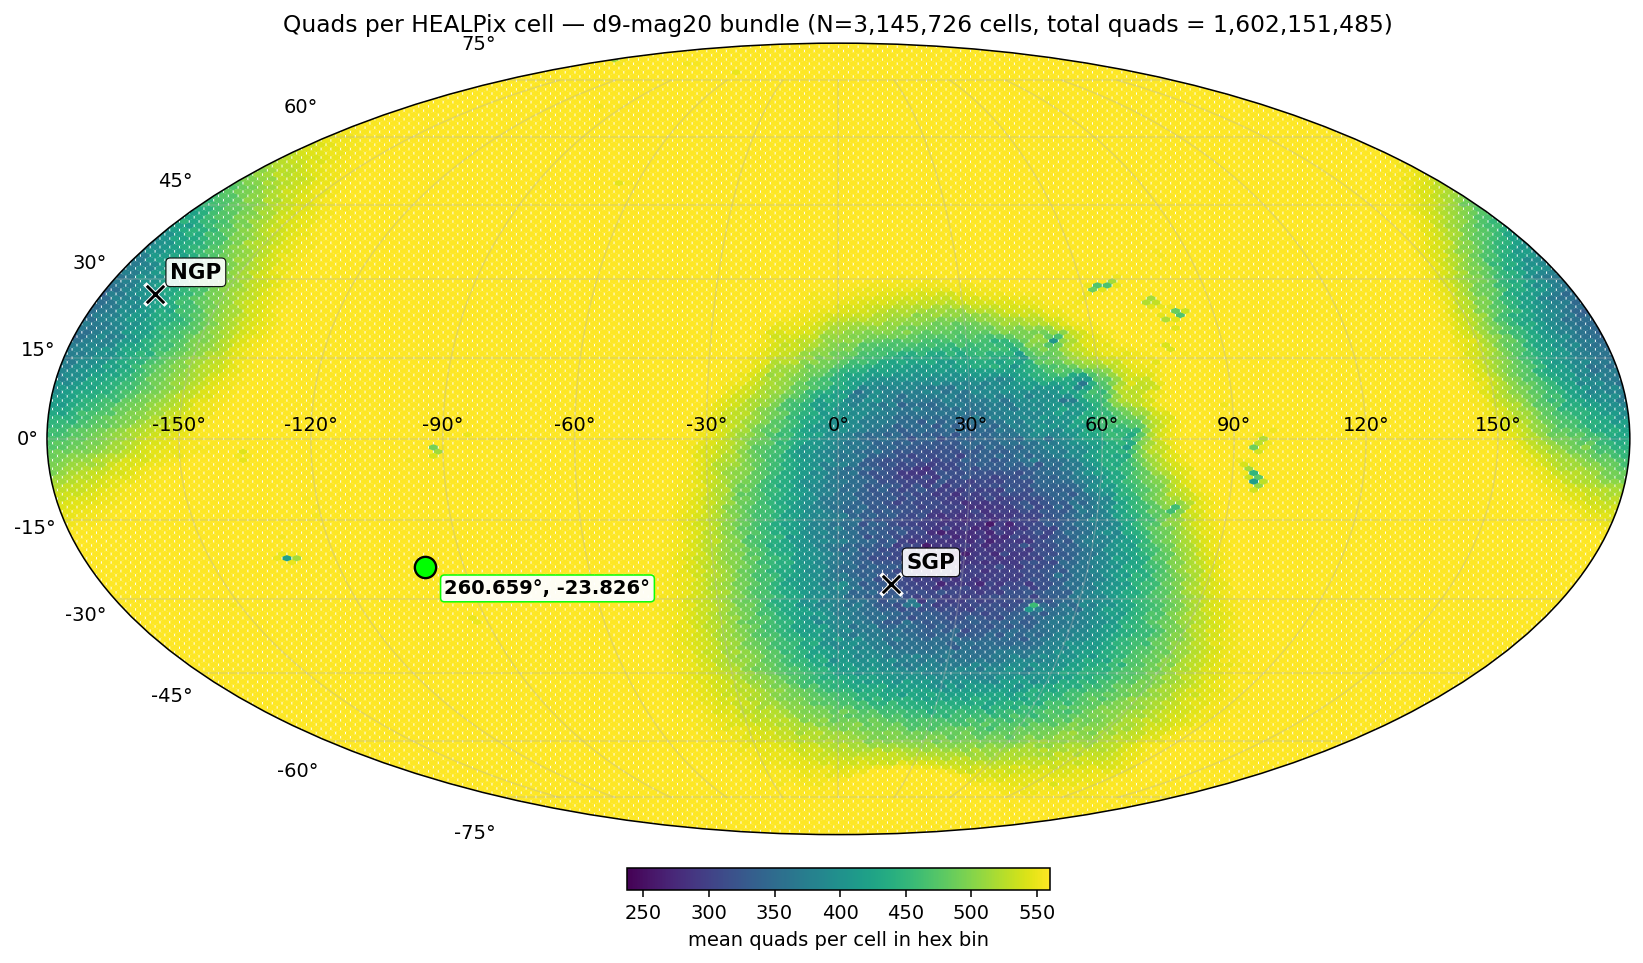
\includegraphics[width=\columnwidth]{figures/d9_quads_per_cell_mollweide.png}
\caption{\label{fig:d9_quads_per_cell} Mean quads per HEALPix cell
across the sky for the depth-9, $G \le 20$ bundle ($N = 3{,}145{,}726$
populated cells, total $1.60\times 10^9$ quads). The cap of 560
quads/cell ($80 \times 7$ bands) is saturated across the entire
plane and high-latitude sky; the Galactic poles (NGP and SGP marked)
are the only regions where the per-cell quad-builder runs out of
candidate stars before reaching the cap. Cell area is computed
analytically from \texttt{.zqd} file sizes via the relation
$n_q = (s - 200)/48$, requiring no catalog access.}
\end{figure}

\subsection{Region-Restricted Solving} \label{sec:region-solve}

The query API takes a \texttt{SkyRegion(centre, radius)}.
\texttt{ZdclBundle::load\_region} enumerates the cells whose centres
fall within $R + r_\text{cell}$ of the hint and hands the solver a
fragment that contains only those cells' quads/codes/stars. For an
IMX455-class FOV with a tight pointing prior the hint can be the
truth pointing $\pm$ a few arcminutes; for a coarse all-sky-mode
solve, $R$ is the full $\pi$\,radians and the bundle reader pages
through all 3.1\,M cells via the LRU-bounded mmap cache.

Because both bundle-side caches---the per-cell shard cache in
\texttt{ZdclBundle} and the per-entry mmap cache in
\texttt{FsAccessor}---use bounded \texttt{LruCache}s, repeated
queries against the same bundle do not leak memory: a 1000-case
sweep at $R = 4\degr$ holds approximately
$\min($workers~$\times$~cells/region, cache cap$)$ entries
resident, which on the test bench peaks around 4\,GB regardless of
sweep length.

\subsection{Empirical Performance vs. Pointing-Hint Radius}
\label{sec:bundle-results}

We characterise the speed/accuracy trade-off as a function of hint
radius using the 1000-case \texttt{set2-dr3-mag19} corpus (described
in §\ref{sec:testconfig}, regenerated against the depth-9 bundle).
Each case is solved with the bench's regional + scale-hinted
configuration ($\pm 25$\% scale tolerance) at four radii: $0.5\degr$,
$1.0\degr$, $2.0\degr$, $4.0\degr$. The cells loaded per query scale
as $\pi R^2 \cdot 76.3$ (cells per square degree at $d_b{=}9$), giving
roughly $60$, $240$, $960$, and $3800$ cells per region respectively.

\textbf{Solve rate: 100\% across all four radii.} The findability
fix from §\ref{sec:fov-aware} closes the depth-8 failure mode
entirely; every test case in the corpus passes the
\texttt{log\_odds\_accept}~$=~20$ threshold at every hint radius
tested.

\textbf{Solve time scales near-linearly with $R$.} Median solve time
is 1.0\,ms at $R = 0.5\degr$, rising to 12.85\,ms at $R = 4\degr$
(Fig.~\ref{fig:d9_solve_cdf}). The median tracks the radius rather
than the area because the solver locks onto the correct hypothesis
in its first few quad-code matches; what scales with the loaded cell
count is the long tail (p99 grows from 18\,ms to 563\,ms, a 30$\times$
spread).

\begin{figure}[t]
\centering
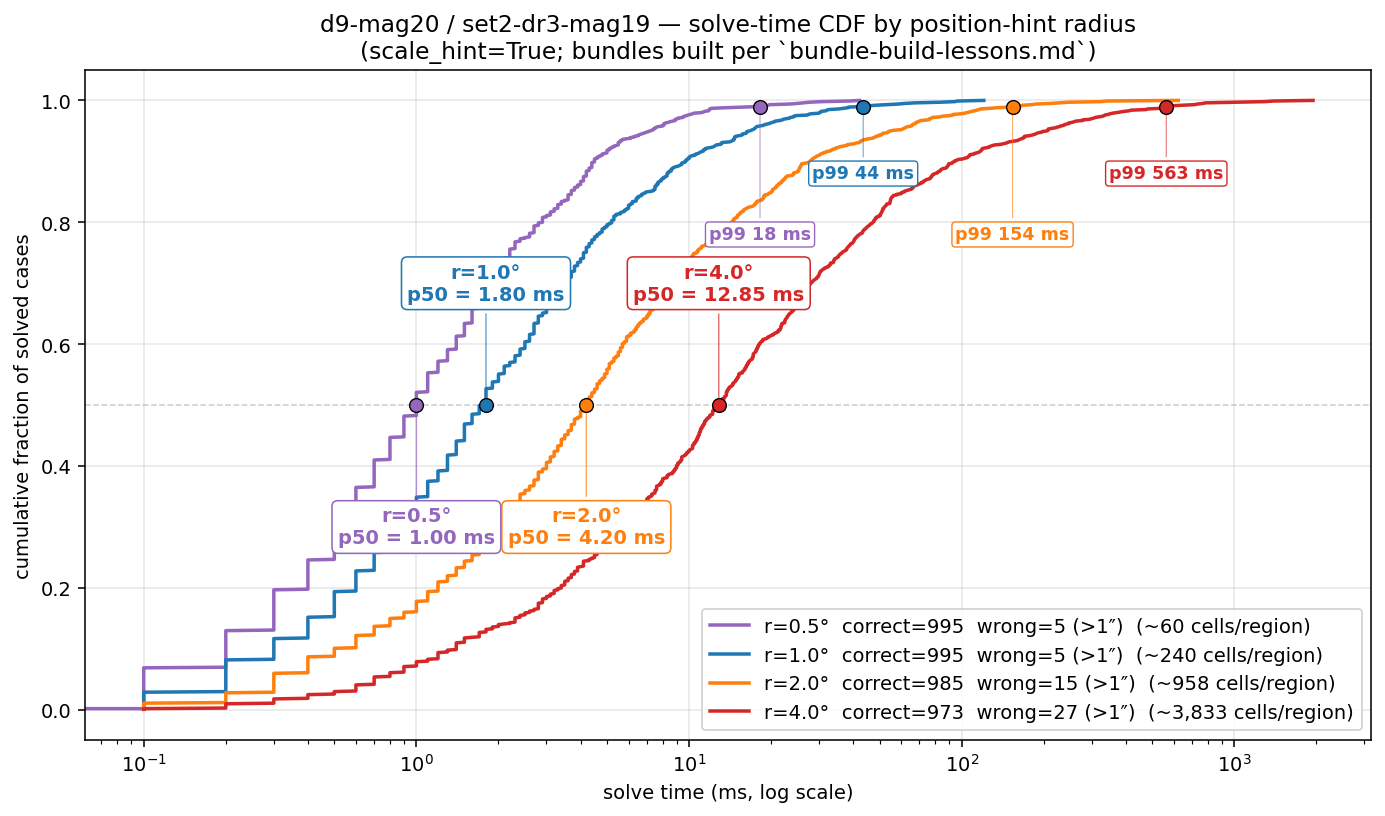
\includegraphics[width=\columnwidth]{figures/d9_solve_time_by_radius_cdf.png}
\caption{\label{fig:d9_solve_cdf} Solve-time CDF at four pointing-hint
radii against the depth-9 bundle. Each curve is 1000 cases. p50 and
p99 callouts shown; the count of approximate cells loaded per query
appears in the legend.}
\end{figure}

\textbf{Region-load time scales as $R^2$.} Median load grows from
22\,ms at $R = 0.5\degr$ to 2.5\,s at $R = 4\degr$
(Fig.~\ref{fig:d9_load_cdf}); the p99 tail balloons from 430\,ms to
34\,s, dominated by dense Galactic-plane regions whose per-cell
shards are 5--10$\times$ larger than the average. Load time is a
direct function of cells touched and is the dominant cost at large
hints---above $R \approx 1\degr$ the bundle read overtakes the solve
itself.

\begin{figure}[t]
\centering
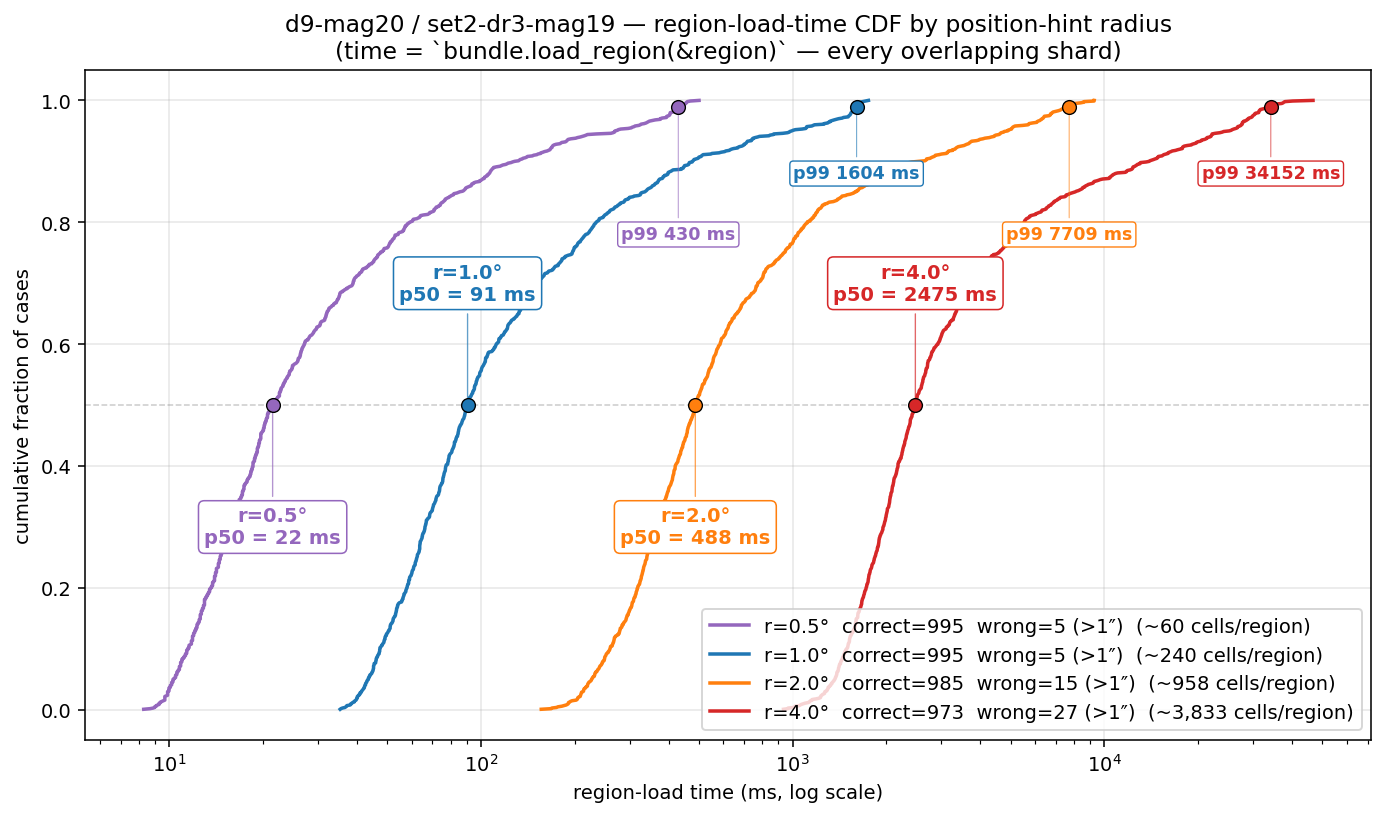
\includegraphics[width=\columnwidth]{figures/d9_load_time_by_radius_cdf.png}
\caption{\label{fig:d9_load_cdf} Region-load-time CDF (the cost of
\texttt{bundle.load\_region(\&region)} per case). Scales as $R^2$
because loaded cell count scales as $R^2$; p99 tail is dominated by
dense Galactic-plane regions.}
\end{figure}

\textbf{Accuracy: median 4\,milliarcsec, with a tail at large $R$.}
The angular-distance error between the solver's WCS centre and the
truth pointing has a median of 0.004\arcsec\ at every hint radius
(Fig.~\ref{fig:d9_acc_cdf})---when the solver finds the right
hypothesis, accuracy is set by Gaia catalog precision and the
WCS-fit residual rather than by the size of the search region. The
\emph{tail}, however, splits dramatically: at $R \le 1\degr$ the p99
error stays at 0.34\arcsec, but at $R = 2\degr$ it jumps to
3557\arcsec\ and at $R = 4\degr$ to 9722\arcsec\ ($\approx
2.7\degr$). These are not solver "failures" in the traditional
sense---they pass the log-odds verification threshold---they are
false-positive WCSes drawn from elsewhere in the loaded region.
Counted as wrong-solves above 1\arcsec, the rates are 0.5\% / 0.5\%
/ 1.5\% / 2.7\% across the four radii.

\begin{figure}[t]
\centering
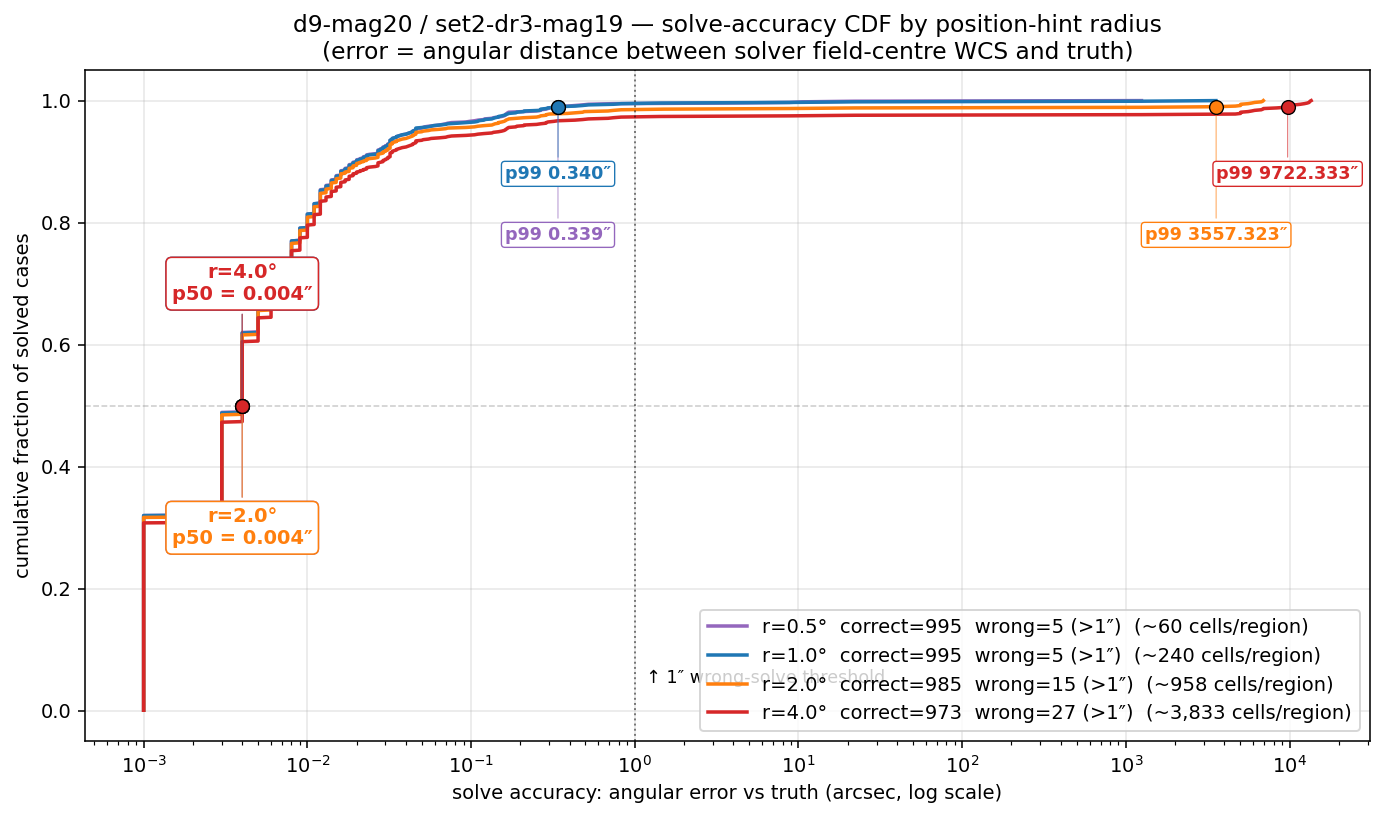
\includegraphics[width=\columnwidth]{figures/d9_accuracy_by_radius_cdf.png}
\caption{\label{fig:d9_acc_cdf} Solve-accuracy CDF. Median accuracy is
hint-radius-independent at $\sim$4\,mas; the p99 tail diverges
sharply at $R \ge 2\degr$, populated by false-positive WCSes that
nonetheless pass the log-odds threshold. The vertical dashed line is
our 1\arcsec\ wrong-solve threshold.}
\end{figure}

The signed (RA, Dec) residuals for the correct cluster
(Fig.~\ref{fig:d9_radec_hists}) are well-centred on zero
($|\text{mean}| < 2$\,mas) with $\sigma_{\Delta\alpha\cos\delta} =
32$\,mas and $\sigma_{\Delta\delta} = 46$\,mas. The slight asymmetry
between the two axes is the characteristic signature of TAN-WCS
least-squares fitting: the dec axis has tighter geometric coupling
than the cos$\delta$-scaled RA component.

\begin{figure}[t]
\centering
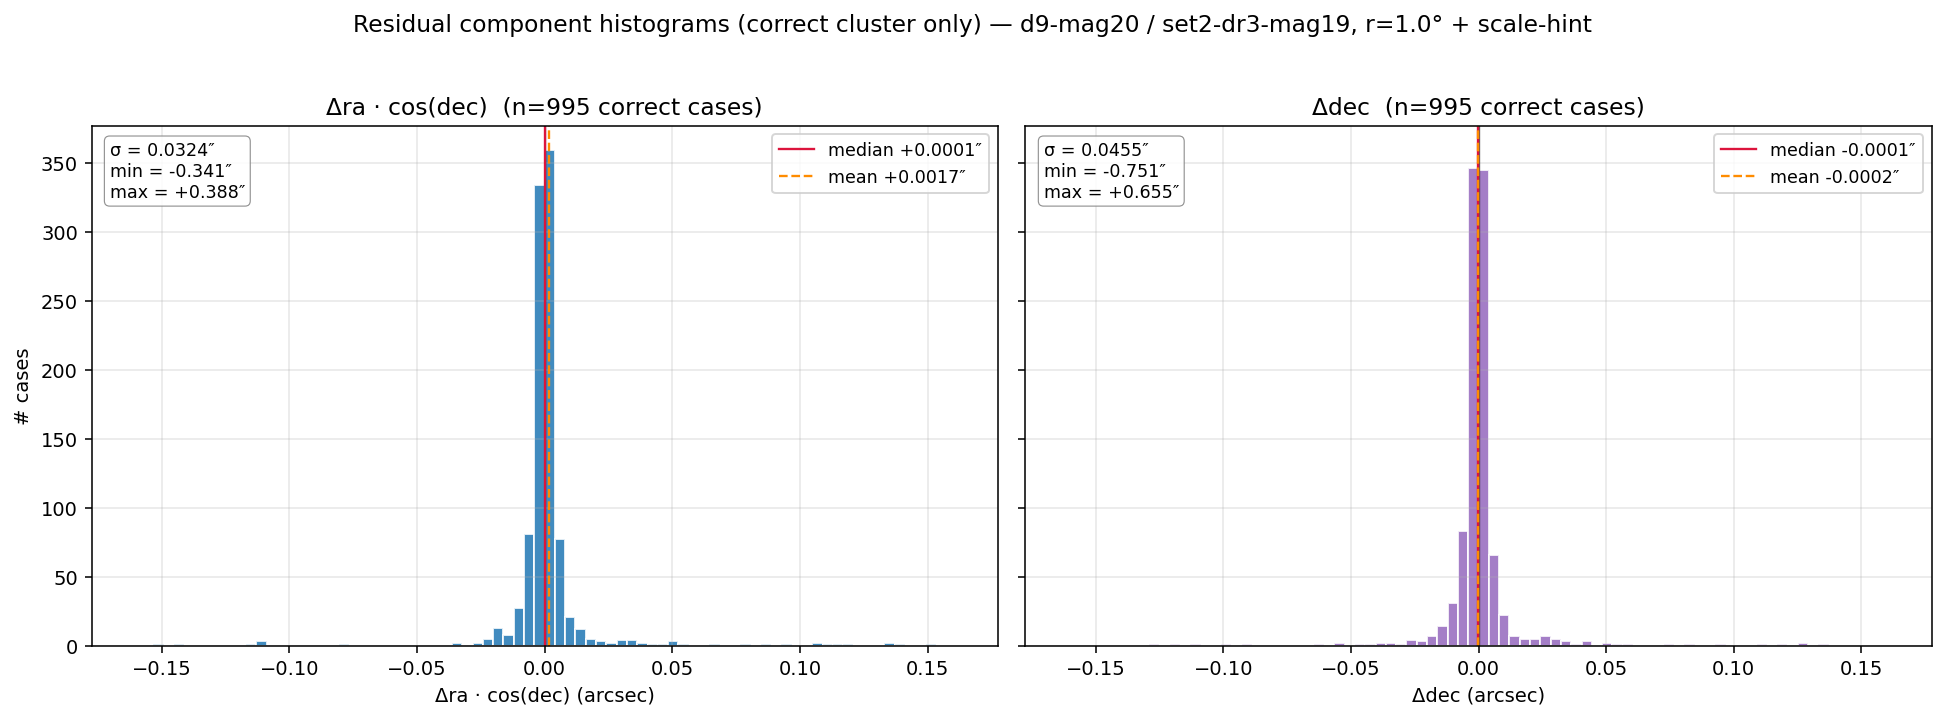
\includegraphics[width=\columnwidth]{figures/d9_radec_residual_hists_r1.png}
\caption{\label{fig:d9_radec_hists} Histograms of the signed RA and
Dec residual components for the 995 correct cases at $R = 1\degr$
(error $\le$ 1\arcsec). Both centred at zero to within 2\,mas;
$\sigma_{\Delta\alpha\cos\delta} = 32$\,mas, $\sigma_{\Delta\delta} =
46$\,mas. Larger Dec scatter reflects TAN-WCS fitting geometry.}
\end{figure}

\textbf{Wrong-solve geography.} The wrong-solve cases are
distributed across the sky but biased toward low-quad-density
Galactic-pole regions (Fig.~\ref{fig:d9_failures}), which is
consistent with the failure mechanism: at high $|b|$, the bundle
holds fewer correct quads in the loaded region, so the relative
weight of code-tolerance-passing spurious matches goes up.

\begin{figure}[t]
\centering
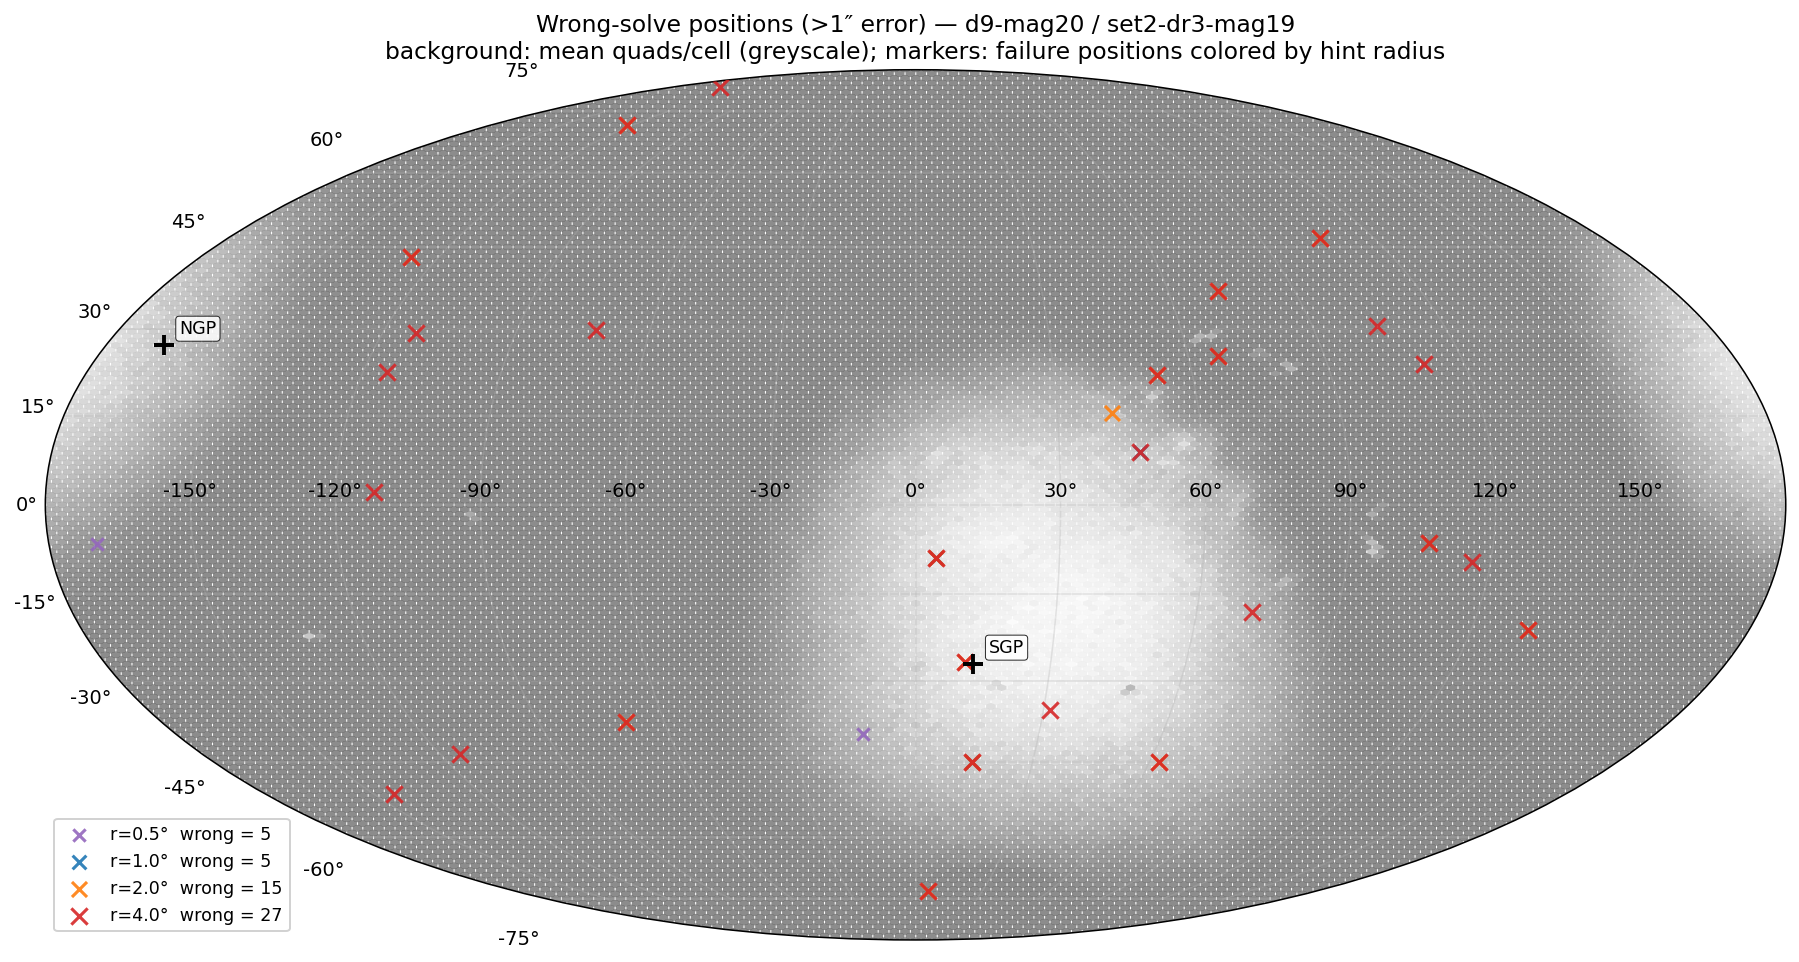
\includegraphics[width=\columnwidth]{figures/d9_failures_mollweide.png}
\caption{\label{fig:d9_failures} Wrong-solve case locations (error
$>$ 1\arcsec) for all four hint radii against the depth-9 bundle.
Background greyscale shows quads-per-cell density.
Wrong-solve concentrations near the Galactic poles trace the
catalog's lowest-density regions.}
\end{figure}

\subsection{Practical Implications} \label{sec:bundle-implications}

Operationally, the bundle format reduces the all-sky deep
($G \le 20$) catalog from a multi-tens-of-GB single index to a 171\,GB
2D-sharded structure that is mmap-friendly, queryable in
milliseconds-to-seconds depending on the hint, and survives long
build pipelines on commodity hardware. The hint-radius/solve-time
trade space is a useful operational dial: pipelines with a ground
truth pointing within $\pm 30\arcmin$ should expect 1--2\,ms median
solves and zero false positives, while wider-area surveys with only
degree-scale priors should accept the sub-percent false-positive
rate or layer a post-solve sanity check (e.g., requiring residual
RMS $\le$ catalog precision) on top of the log-odds verification.

\subsection{Bounded Caches for Long-Running Services}
\label{sec:bounded-caches}

The radius sweep in \S\ref{sec:bundle-results} exposed a stability
problem inherent to mmap-backed bundle access. Both the per-cell
shard cache in \texttt{ZdclBundle} and the per-entry mmap cache in
the underlying \texttt{FsAccessor} were initially unbounded
\texttt{HashMap}s: once a cell was touched, its quad and Gaia bytes
stayed mapped for the lifetime of the bundle handle. For a 1000-case
sweep at $R = 5\degr$ this is roughly $10^{6}$ cells $\times$
${\sim}30$\,kB/cell ${\approx}$~45\,GB of cumulative mappings;
the process \texttt{malloc}'d to death at case 92.

Both caches are now \texttt{LruCache}s with a configurable capacity
(default $10^{5}$ entries). The eviction-safety subtlety is in
\texttt{FsAccessor}: the public read API previously returned a slice
borrowed into the cached \texttt{Box<Mmap>} and relied on entries
never being removed. We changed the cached value to \texttt{Arc<Mmap>}
and the return type from \texttt{\&[u8]} to an \texttt{EntryBytes}
enum whose mmap variant carries an \texttt{Arc} clone. Callers that
still hold an \texttt{EntryBytes} keep the underlying mapping alive
through their \texttt{Arc} even after the cache evicts the entry,
preserving the zero-copy fast path on the hot path while allowing
the LRU to do its job. With both caches bounded, the sweep at
$R = 4\degr$ now completes in $\sim$4\,GB peak resident set, set by
the cache cap rather than by sweep length.

\subsection{Per-Case Solver Traces and Diagnostic Tooling}
\label{sec:solver-trace}

The Bayesian verifier's output is a scalar log-odds; when a quad
that ``should have'' matched is rejected, that scalar gives no
visibility into \emph{why}. To support post-mortem analysis on real
imagery, the bench harness can optionally emit a per-case
\texttt{<case>.trace.json} sidecar containing the fitted WCS, the
matched quad's four \texttt{(field, catalog)} pairs (with the
index-band identifier that produced the match), and the full
verification matched-pair list. A companion Python renderer overlays
all of that on the original FITS image: catalog stars projected
through the recovered WCS, detection-side sources, the four backbone
vertices, and per-pair connection segments clipped at vertex disks.

The renderer was developed specifically to investigate verification
failures on HST archival fields and surfaced the proper-motion
mismatch described in \S\ref{sec:pm}: at high enough proper motion,
a real detection's match to the right catalog star can fall outside
the verifier's match radius purely because the catalog position is
fixed at the Gaia DR3 epoch. The trace renderer made the
displacement immediately visible as a systematic offset between
detected and projected positions for the misclassified star,
motivating the epoch-aware verifier change that this paper's
\S\ref{sec:pm} measures end-to-end.

% =============================================================================
\section{Proper Motion at the Observation Epoch} \label{sec:pm}
% =============================================================================

The bundle results in \S\ref{sec:bundle-results} were measured against
the \texttt{set2-dr3-mag19} corpus, which is synthesised at Gaia DR3's
reference epoch ($J2016.0$). For survey pipelines operating close to
that epoch the simplification is harmless: stellar drift over a few
years stays well below a typical 5\,px match radius. Out-of-epoch
plates---most acutely \emph{archival} Hubble Space Telescope frames
spanning $\sim$1990--2015, but also any pipeline asked to register an
image to a time-of-flight epoch---break this assumption. A nominally
500\,mas\,yr$^{-1}$ star drifts 7\arcsec\ in 14 years; on a Hubble ACS
0.05\arcsec/px plate that is 140\,px and the verifier will not
associate the detection with the catalog entry at all.

Zodiacal handles this by carrying per-star proper motion through the
index and applying it at both read sites that turn $(\alpha, \delta)$
into a sky vector: the quad-to-WCS fit
(\S\ref{sec:fitting}) and the Bayesian verification pass
(\S\ref{sec:verify}). The on-disk \texttt{.zga} per-cell Gaia shard
(\S\ref{sec:bundle-format}) already carries the full DR3 astrometric
solution (\texttt{pmra}, \texttt{pmdec}, reference epoch); enabling
this path required only widening the in-memory \texttt{IndexStar}
record from 4 to 7 fields and threading an \texttt{Option<f64>}
observation epoch through the solver configuration.

\subsection{Linear Small-Angle Extrapolation} \label{sec:pm-prop}

The extrapolation is the standard linear form, applied independently
to each axis:
\begin{align}
    \alpha(t_{\text{obs}}) &= \alpha(t_{\text{ref}})
        + \mu_{\alpha^*} \cdot \frac{t_{\text{obs}} - t_{\text{ref}}}
        {\cos \delta(t_{\text{ref}})}, \label{eq:pm-ra} \\
    \delta(t_{\text{obs}}) &= \delta(t_{\text{ref}})
        + \mu_{\delta} \cdot (t_{\text{obs}} - t_{\text{ref}}), \label{eq:pm-dec}
\end{align}
where $\mu_{\alpha^*} \equiv \mu_{\alpha} \cos \delta$ is the Gaia
true-sky RA proper motion in mas\,yr$^{-1}$, the time difference is in
Julian decimal years, and the inverse $\cos \delta$ converts the
true-sky rate into a coordinate rate. For fast-moving stars
($\mu \sim 5{,}000$\,mas\,yr$^{-1}$) over decade-scale gaps this is
accurate to $\sim 10\,\mu$as---two orders of magnitude below any
pixel tolerance we care about. Parallax, light-time, and stellar
aberration are not applied at the solver level; the \texttt{refinement}
module's apparent-place pipeline picks those up for follow-up
astrometry once a WCS is in hand.

Two practical guards keep this robust against legacy data. Catalog
entries with NaN proper motion---Gaia DR3's 2-parameter solutions, and
all stars in pre-bundle \texttt{.zdcl} v1/v2 indexes---are returned
unchanged, so a missing measurement degrades silently to the identity
rather than corrupting the position with NaN propagation. The
observation epoch is itself optional: passing \texttt{None} bypasses
\eqref{eq:pm-ra}--\eqref{eq:pm-dec} entirely and the verifier behaves
bit-identically to the pre-PM solver. Synthetic Gaia-epoch corpora
therefore continue to produce the same outcomes as
\S\ref{sec:bundle-results}.

\subsection{Recovering a High-Proper-Motion Star} \label{sec:pm-recovery}

A regression test in \texttt{src/verify.rs} pins the behaviour with
a worked instance. A synthetic detection is placed at pixel
$(300, 400)$ under a 1\arcsec/px WCS, and the catalog entry is
back-extrapolated from a 14-year-distant observation epoch using a
$500$\,mas\,yr$^{-1}$ proper motion. The forward drift between
epochs is $7000$\,mas $= 7$\,px, outside the default $5$\,px match
radius:

\begin{itemize}
    \item \textbf{Without} \texttt{obs\_epoch}: the verifier projects
          the index's 2016 position, lands $\sim 7$\,px from the
          detection, and the star is unmatched.
    \item \textbf{With} \texttt{obs\_epoch}: the projection
          first applies Eqs.~\ref{eq:pm-ra}--\ref{eq:pm-dec} to roll
          the position forward to the observation epoch, lands inside
          the match circle, and the star contributes its
          $\Delta_i \gtrsim 0$ to the log-odds total.
\end{itemize}

The same wiring is used by \texttt{zodiacal-tools bench-bundle}, which
gained an \texttt{--obs-epoch} flag and an automatic Hubble path that
fills \texttt{obs\_epoch} from the test case's \texttt{t\_min\_mjd}/
\texttt{t\_max\_mjd} midpoint. HST plates therefore solve without
operator intervention against a Gaia-epoch bundle, and the bundle on
disk gains no new fields.

\subsection{When Proper Motion Matters in Practice} \label{sec:pm-when}

The pixel-scale drift admissible without proper-motion correction is
\begin{equation} \label{eq:pm-budget}
    \Delta t \lesssim \frac{r_{\text{match}} \cdot s_{\text{px}}}
                            {\mu_{\text{cap}}},
\end{equation}
where $r_{\text{match}}$ is the verifier match radius (default
$5$\,px), $s_{\text{px}}$ is the plate scale, and
$\mu_{\text{cap}}$ is the proper motion above which a star
contributes to verification failures. At the bench's
0.1296\arcsec/px and the $\sim$1\,\% of Gaia DR3 stars with
$\mu > 100$\,mas\,yr$^{-1}$, the budget is $\sim 6.5$\,years before
high-PM stars start dropping out of the match circle. At HST/ACS's
0.05\arcsec/px it shrinks to $\sim 2.5$\,years. Pipelines registering
images more than this far from the catalog epoch should set
\texttt{obs\_epoch}; pipelines within the budget see no behavioural
change either way.

% =============================================================================
\section{Conclusion} \label{sec:conclusion}
% =============================================================================

We have presented Zodiacal, a pure-Rust blind astrometry plate solver
that achieves 98.3\% solve rates with a median time of 1.42\,s on
simulated narrow-field imagery. Our systematic evaluation of index
sharding strategies demonstrates that partitioning the angular scale
space into narrow bands is a first-order design decision: moving from
4 coarse bands to 12 fine bands ($\sqrt{2}$ scale factor) improves
the solve rate by 2.3 percentage points while maintaining sub-second
median solve times for the majority of fields.

The performance benefit arises from two mechanisms: smaller per-band
$k$-d trees that reduce false-positive code matches, and per-index
scale filtering that prunes irrelevant bands entirely. These combine
to reduce the effective search space by an order of magnitude for
typical fields.

The residual 1.7\% failure population is characterized by
large-backbone geometries that produce code-space collisions,
representing a search budget challenge for geometric hashing
approaches that narrower bands alone cannot fully resolve.

The legacy single-index design also bounds catalog depth to what
fits in working RAM. \S\ref{sec:bundle} lifts that limit by adding a
second sharding axis: the \texttt{.zdcl.bundle} format pairs
per-cell HEALPix shards with the existing scale-band split, and the
bundle reader loads only the cells overlapping a user-supplied sky
region. Against a depth-9, $G \le 20$ bundle ($\sim$$9 \times 10^8$
stars, 1.6$\times 10^9$ quads) and the \texttt{set2-dr3-mag19}
1000-case corpus, this delivers a 100\% solve rate, 1--13\,ms median
solve time depending on hint radius, and median 4\,milliarcsec
positional accuracy. We characterise the speed/accuracy trade-off
across hint radii of $0.5\degr$--$4.0\degr$, including the
false-positive WCS regime that emerges at large radii where multiple
quads can plausibly verify the same field.

Out-of-epoch plates are handled by \S\ref{sec:pm}: per-star proper
motion is carried through the bundle's \texttt{.zga} shards and
applied at WCS fit and verification when the caller supplies an
observation epoch. The solver continues to behave bit-identically to
the pre-PM path when no epoch is given, so synthetic Gaia-epoch
corpora are unaffected; archival HST plates now solve against the
same depth-9 bundle without operator intervention.

Zodiacal is open-source and available at
\url{https://github.com/OrbitalCommons/zodiacal}.

\section*{Acknowledgments}

This work makes use of data from the European Space Agency mission
Gaia (\url{https://www.cosmos.esa.int/gaia}), processed by the Gaia
Data Processing and Analysis Consortium.

\bibliographystyle{plainnat}
\bibliography{zodiacal}

\end{document}
